%%%%%%%%%%%%%%%%%%%%%%%%%%%%%%%%%%%%%%%%%
% Thin Sectioned Essay
% LaTeX Template
% Version 1.0 (3/8/13)
%
% This template has been downloaded from:
% http://www.LaTeXTemplates.com
%
% Original Author:
% Nicolas Diaz (nsdiaz@uc.cl) with extensive modifications by:
% Vel (vel@latextemplates.com)
%
% License:
% CC BY-NC-SA 3.0 (http://creativecommons.org/licenses/by-nc-sa/3.0/)
%
%%%%%%%%%%%%%%%%%%%%%%%%%%%%%%%%%%%%%%%%%

%----------------------------------------------------------------------------------------
%	PACKAGES AND OTHER DOCUMENT CONFIGURATIONS
%----------------------------------------------------------------------------------------

\documentclass[a4paper, 12pt]{article} % Font size (can be 10pt, 11pt or 12pt) and paper size (remove a4paper for US letter paper)

\usepackage[protrusion=true,expansion=true]{microtype} % Better typography
\usepackage[frenchb]{babel}
\usepackage{graphicx} % Required for including pictures
\usepackage{wrapfig} % Allows in-line images

\usepackage{mathpazo} % Use the Palatino font
\usepackage[utf8]{inputenc} % UTF-8 encoding for input, to get french special characters recognized
\usepackage[T1]{fontenc} % Required for accented characters
\linespread{1.05} % Change line spacing here, Palatino benefits from a slight increase by default
\usepackage{parskip} % add some space between paragraph 
\usepackage{pdfpages}
 
\makeatletter
\renewcommand\@biblabel[1]{\textbf{#1.}} % Change the square brackets for each bibliography item from '[1]' to '1.'
\renewcommand{\@listI}{\itemsep=0pt} % Reduce the space between items in the itemize and enumerate environments and the bibliography

\renewcommand{\maketitle}{ % Customize the title - do not edit title and author name here, see the TITLE block below
\begin{flushright} % Right align
{\LARGE\@title} % Increase the font size of the title

\vspace{50pt} % Some vertical space between the title and author name

\vspace{40pt} % Some vertical space between the author block and abstract
\end{flushright}
}

\begin{document}

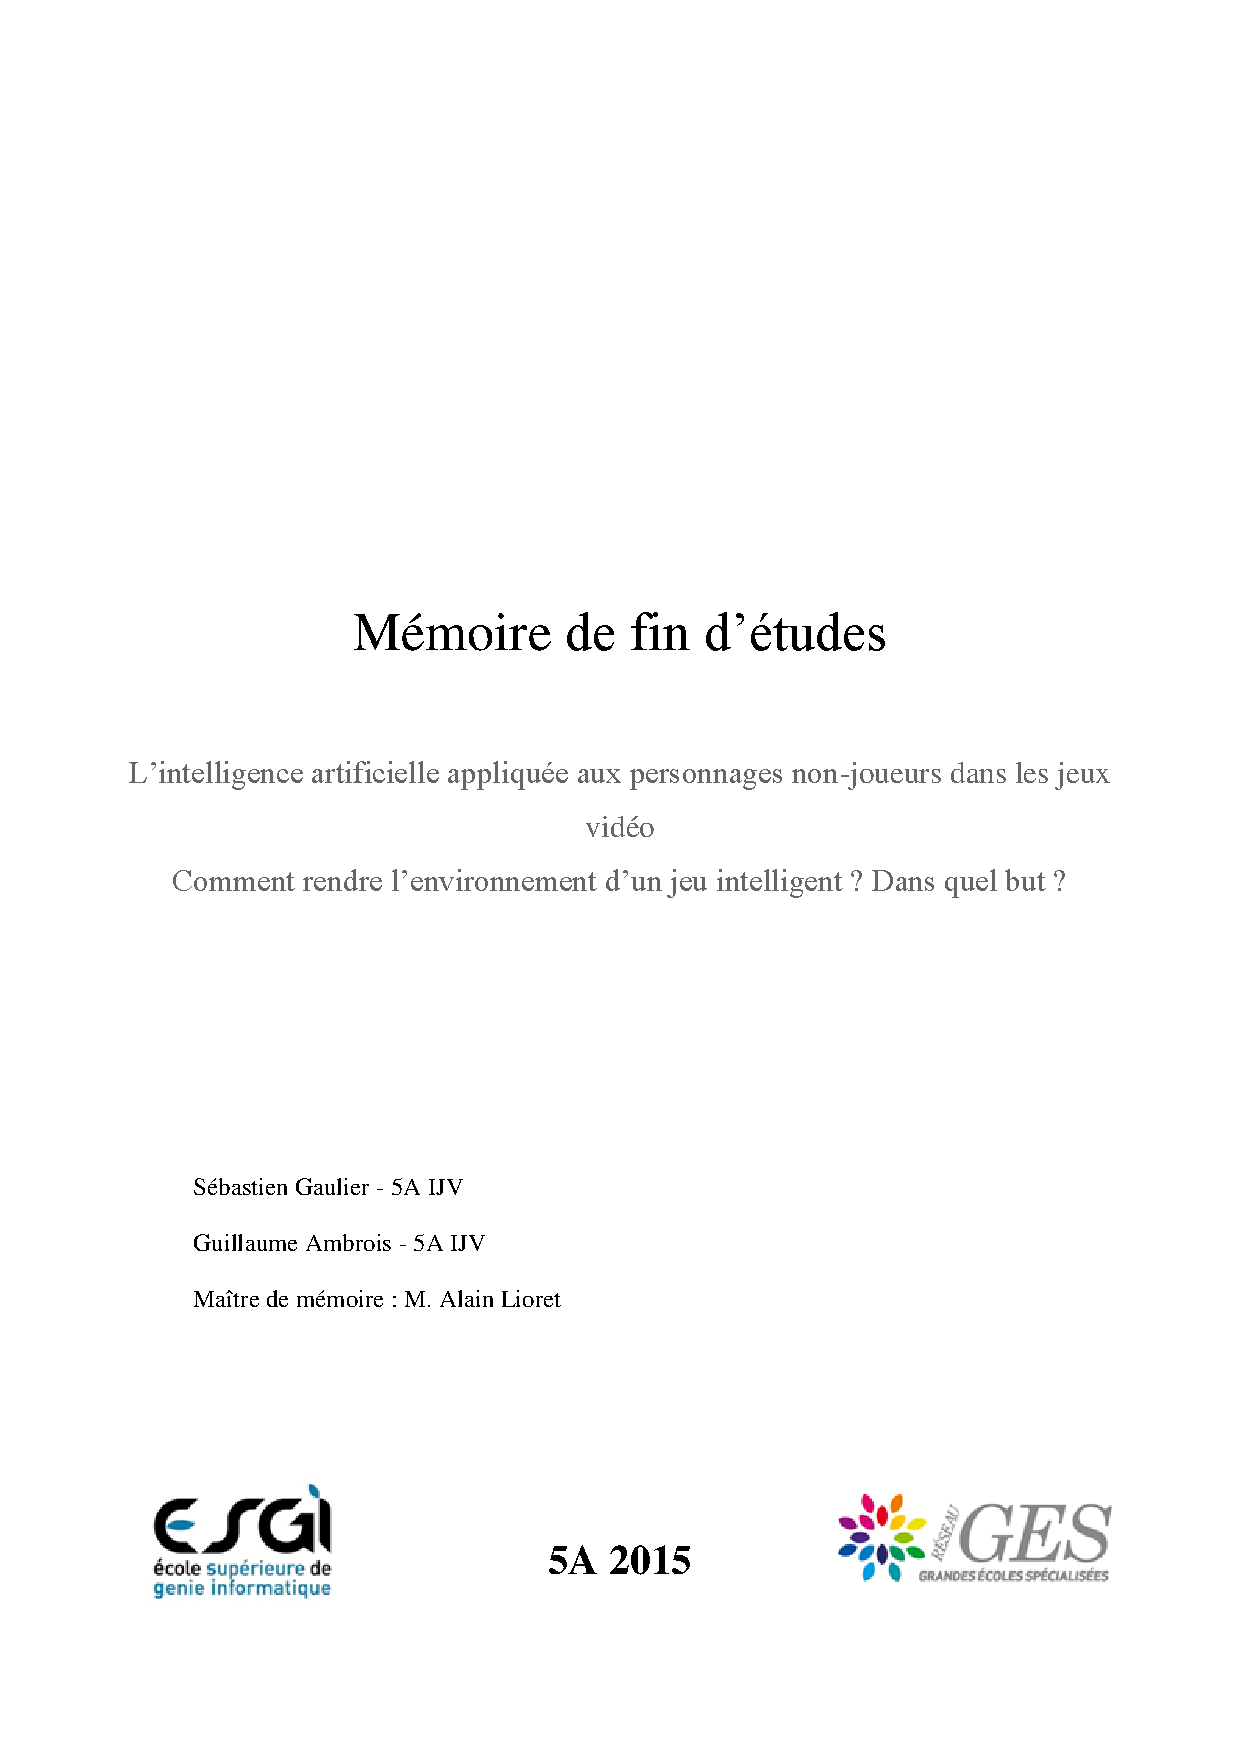
\includepdf[pages={1}]{images/pagedegarde.pdf}

%----------------------------------------------------------------------------------------
%	ESSAY BODY
%----------------------------------------------------------------------------------------

\tableofcontents
\newpage
\section{Avant-propos}
\subsection{Remerciements}
Nous tenons à remercier :

M. Alain LIORET, notre maître de mémoire, pour son soutien, sa passion, et pour nous avoir guidé dans notre travail. Il nous a donné de très bonnes pistes de recherches, et a su nous conseiller dans nos choix.

L’équipe pédagogique de l’ESGI, pour la qualité de leurs cours, qui nous ont donné la motivation nécessaire pour rédiger ce mémoire.

\newpage
\subsection{Résumé}
Les jeux vidéo sont de plus en plus beaux, que ce soit en approchant le photoréalisme, ou en ayant une patte graphique unique. Ils sont également de plus en plus profonds, avec une histoire, une narration et un univers toujours plus poussés. Le gameplay également n’a de cesse de s’améliorer, que ce soit à travers de nouvelles idées innovantes de game design, ou via de nouveaux périphériques pour renforcer l’interaction ainsi que l’immersion du joueur. 

Mais le domaine dans lequel il reste le plus de progrès à faire pour proposer des expériences toujours plus intéressantes et immersives est l’intelligence artificielle (IA). Bien que celle-ci soit de plus en plus présente (et attendue) dans les jeux, et de plus en plus évoluée grâce à des algorithmes toujours plus performants, cela reste en général une IA « fixe », avec des comportements prévus à l’avance, en réponse à des évènements prévus à l’avance.

En effet, bien souvent les personnages non joueurs (PNJ) sont des entités statiques du jeu ne possédant qu’un panel fixe d’actions ou de répliques de dialogues, qu’ils soient alliés (marchand), ou ennemis (monstre). Ces personnages sont ainsi relégués au rang d’élément du décor, alors qu’ils pourraient occuper une place bien plus importante dans le jeu, apportant à la fois en profondeur de gameplay et de narration.

Dans ce mémoire, nous étudierons les différentes IA qui existent actuellement, ainsi que ce qu’elles apportent en termes d'expérience.

\newpage
\subsection{Abstract}
Video games are more and more beautiful, whether it be by approaching photorealism, or by using a unique graphic style. They’re also more and more deep, with a story, a narration and an universe always more advanced. The gameplay keeps getting better, either with innovative game design ideas, or with new devices to enhance the interaction and immersion of the player.
 
But there is a field in which much progresses are yet to be done in order to offer ever more interesting and immersive experiences, and this field is artificial intelligence (AI). Although it’s more and more present (and expected) in video games, and more and more efficient through algorithms ever more powerful, it remains, in general a scripted AI, with programmed behaviors which respond to specific events. 

Indeed, often the non-player characters (NPCs) are static entities of the game with only a fixed panel of actions or dialogues replicas, whether allies (merchant) or enemies (monster). These characters are relegated to the role of decorative elements, when they could take a more important place in the game, providing both depth of gameplay and storytelling.
In this thesis, we will study the state of the art of artificial intelligence applied on NPCs, and what they offer in term of experience.

\newpage
\subsection{Mots clés}
\begin{center}
	\begin{tabular}{|p{0.45\columnwidth}|p{0.45\columnwidth}|}
		\hline
		Mots clés & Key words\\
		\hline		
		Intelligence Artificielle			&Artificial Intelligence\\
		Jeu vidéo							&Video game\\
		Personnage Non Joueur (PNJ)			&Non Playable Character (NPC)\\
		Apprentissage Automatique			&Machine Learning\\
		Réseaux de neurones					&Neural Networks\\
		Dynamic Game Difficulty Balancing	&Dynamic Game Difficulty Balancing\\
		General Video Game Playing			&General Video Game Playing\\
		\hline
	\end{tabular}
\end{center}

\newpage
\section{Introduction}
Depuis leur invention, les jeux vidéo n’ont eu de cesse de s’améliorer, que ce soit du point de vue du gameplay, du scénario ou du matériel. Mais un aspect qui est reste encore aujourd’hui en retrait (en plus du fait que lorsqu’elle est bien réalisée, elle est discrète), c’est l’intelligence artificielle.
 
Un premier problème se situe au niveau de la crédibilité du comportement, empêchant le joueur de s'immerger totalement. C’est une problématique impactant principalement les jeux solos. En effet, le cœur des jeux vidéo se jouant seul est son scénario. Il est donc nécessaire que l’histoire ainsi que ses personnages paraissent le plus crédible possible aux yeux du joueur.

Un deuxième problème se situe au niveau du degré de compétences de l’IA. En effet, celui-ci est souvent fixe, défini à l’avance, et impersonnel. Il existe plusieurs solutions pour pallier à ce problème, et si quelques jeux utilisent déjà ce genre d’IA un peu plus évoluée (notamment Left 4 Dead et son AI Director, dont nous parlerons plus en détail plus tard), trop peu sont les jeux à les utiliser.

Le constat est donc simple, pour apporter une meilleure expérience au joueur, il faut améliorer le comportement des agents en le rendant plus réaliste d’une part, et plus personnalisable, adaptable, et évolutif d‘autre part.

Il existe beaucoup de types d’IA applicables pour les jeux vidéo, et beaucoup de façon de les réaliser. Nous présenterons dans ce mémoire les principales méthodes, notamment certaines basées autour du Machine Learning, cependant, pour celles-ci, nous restreindrons le champ d’application aux PNJ. 

\newpage
\section{Bref historique de l’IA appliquée aux jeux vidéo}
Dans les jeux vidéo, l’intelligence artificielle est utilisée pour donner vie aux PNJ. Les méthodes employées pour implémenter les algorithmes de ces PNJ s’appuient généralement sur les théories existantes du domaine plus général de l’intelligence artificielle. Cependant, contrairement à une IA classique comme celle d’un robot, l’objectif n’est pas nécessairement de reproduire le comportement d’un humain. Il est même fréquent de voir des PNJ tricher. 

Dans la plupart des jeux, les PNJ ont par exemple connaissance de l’ensemble de la carte et de ce qui s’y déroule. Dans les jeux de type FPS (« First Person Shooter »), les IA sont souvent dotées d’une visée parfaite. Par conséquent, il est très souvent nécessaire de brider ces capacités hors normes pour donner au joueur une sensation d’équité. 

L’histoire de l’IA dans ce domaine remonte au début des années 1940 avec le jeu de stratégie pure Nim (publié en 1942). L’IA était alors capable de gagner, même contre des joueurs chevronnés !

\begin{figure}[!h]%
	\begin{center} 
		
\includegraphics[width=0.60\columnwidth]{images/nim.png}%
		\caption{Le jeu de Nim}%
	\end{center}
\end{figure}

\newpage
\subsection{La naissance de l’IA}
En 1951, les premières IA pour les jeux de Dames et d’Echecs sont créées à partir de la machine Ferranti Mark 1\footnote{Le Ferranti Mark I fut le premier ordinateur électronique généraliste commercialisé du monde. En novembre 1951, Dietrich Prinz écrivit un des premiers jeux vidéo, un programme d’échecs, pour le Ferranti}. Ces IA ont ensuite été améliorées jusqu’à leur point culminant : la défaite du joueur d’Echecs Garry Kasparov, vaincu par le super-ordinateur Deep Blue d’IBM. 

Plus tard entre les années 1960 et le début des années 1970, les premiers jeux développés durant cette période utilisaient la logique discrète et, le plus souvent, n’intégraient pas d’IA car ils opposaient uniquement deux joueurs. 

\begin{figure}[!h]%
	\begin{center} 
		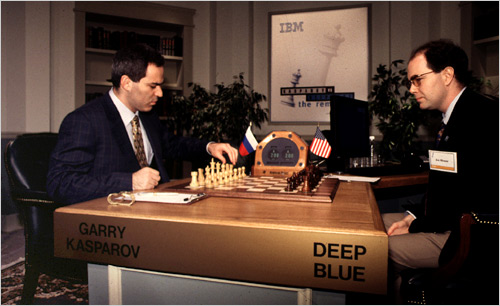
\includegraphics[width=0.60\columnwidth]{images/DeepBlue.png}%
		\caption{Garry Kasparov contre Deep Blue d'IBM}%
	\end{center}
\end{figure}

\newpage
\subsection{Les premières IA pour le jeu vidéo}
Dans les années 1970, les premiers jeux avec des modes 1 joueur apparaissent. Les plus remarquables sont Chasse au Wumpus et Star Trek en 1972 qui utilisaient des Stored Patterns\footnote{Les stored patterns sont des suites d’instructions répétées en boucle par l’agent. Hormis ce qui lui est dit de faire, il ne fera rien d’autre}  pour implémenter les IA des ennemis. L’utilisation des microprocesseurs a permis une augmentation du nombre de mouvement. 

Dans la fin des années 1970 et jusqu’au début des années 1990 : c’est l’âge d’or des jeux d’arcade. Les IA se popularisent. Nombre de jeux (comme Space Invaders en 1978 et Galaxian en 1979) intègrent maintenant une IA plus complexe avec différents niveaux de difficulté et de nombreux modèles de mouvement. 

\begin{itemize}
	\item \textbf{Pacman} (1980) a introduit un pattern IA pour les jeux de labyrinthe, avec des personnalités distinctes pour chaque ennemi.
	\item \textbf{Karate Champ} (1984) a quant à lui introduit le pattern pour les jeux de combat.
	\item \textbf{First Queen} (1988) était un RPG dans lequel des personnages contrôlés par l’IA devaient suivre un leader. Ce type d’IA ayant été amélioré par Dragon Quest IV (1990) avec le system « Tactics » (ajustement des routines utilisées par les IA) puis Secret of Mana (1993).
\end{itemize}

A partir des années 1990, l’émergence de nouveaux genres de jeux vidéo a conduit à l’utilisation d’outils plus sophistiqués tels que les automates finis. Les stratégies en temps réel requéraient la prise en compte de nombreuses contraintes : de nombreux objets, des informations incomplètes, la recherche de chemin, l’économie du nombre de calculs lors de la planification, etc. 

Les premiers jeux rencontraient de nombreux problèmes (Herzog Zwei en 1989 avec une recherche de chemin basée sur un automate fini à trois états, ainsi que Dune 2 en 1992 qui utilisaient de nombreuses « astuces »). 

\newpage
\subsection{Une IA évolutive}

Longtemps délaissée au profit des graphismes des jeux vidéo, cette branche constitue maintenant une part importante du travail dans un jeu vidéo. Les joueurs réclament de plus en plus des IA au comportement humain afin d'accroître le sentiment d’immersion. Certains jeux sont réputés pour être des précurseurs en matière d’IA, en voici quelques exemples : 

\begin{itemize}
	\item \textbf{Creatures} (1998) : ce jeu est célèbre pour être le premier à utiliser l’apprentissage automatique lors d’une simulation interactive. A l’aide des réseaux de neurones, les créatures (appelées « Norms ») apprennent divers comportements. Ils peuvent ainsi interagir avec leur environnement. 

	\item \textbf{Halo : Combat Evolved} (2001) : ce jeu utilisait des arbres pour déterminer le comportement des PNJs (« Behavior Tree »), avec beaucoup d’attention portée sur le moindre détail du jeu. Ainsi, la gestion des groupes de PNJs était particulièrement bonne et a joué un rôle de précurseur. 

	\item \textbf{F.E.A.R.} (2005) : l’IA utilise un planificateur (« Planner ») afin de générer des comportements sensibles au contexte, ce fut la première fois dans un jeu grand public. On ressent une grande habileté chez les PNJs. Ils sont en effet capables de trouver une couverture derrière des tables, basculer des étagères, ouvrir des portes, passer à travers les fenêtres, etc. Ce jeu constitue une référence en la matière.  

	\item \textbf{Black \& White} (2001) : le jeu propose au joueur d’incarner une divinité et de guider un peuple. Pour l’aider dans cette tâche, le joueur devra éduquer sa créature, un agent qu’il sera possible de récompenser après une action pour renforcer ce comportement, ou punir, afin de le diminuer. 
\end{itemize}

\newpage
\section{Les applications possibles prometteuses}

Dans cette section, nous aborderons certaines des techniques les plus utilisées dans les jeux vidéo, plus particulièrement dans le domaine de l’intelligence artificielle. Nous étudierons leurs caractéristiques ainsi que les avantages et les inconvénients de chacune plus particulièrement.

\subsection{Le Machine Learning}

Le Machine Learning est un domaine extrêmement vaste, aussi nous ne parlerons ici que des réseaux de neurones et des arbres de comportement.

\subsubsection{Les réseaux de neurones}

Un réseau de neurones artificiel (RNA) est un paradigme de traitement de l’information qui est inspiré de la façon par laquelle le système nerveux biologique, telle que le cerveau, traite l’information. L’élément clé de ce paradigme est la structure novatrice utilisée pour le système de traitement de l’information. Il est composé d’une grande quantité d’éléments de traitement grandement interconnectés (neurones), qui, en travaillant à l’unisson résolvent des problèmes spécifiques. Les RNA, comme les humains, apprennent par l’exemple. Un RNA est configuré pour une application particulière, comme la reconnaissance de motifs ou la classification de données, à travers une procédure d’apprentissage. Apprendre, dans le système biologique, implique des ajustements au niveau des connections synaptiques qui existent entre les neurones. C’est également vrai pour les RNA.

La simulation de réseaux de neurones apparaît comme étant un développement récent. Cependant, ce domaine a été établi avant l’avènement des ordinateurs, et a survécu à au moins un revers majeur et à plusieurs époques. Le premier réseau de neurones artificiel fût produit en 1943 par le neurophysiologiste Warren McCulloch et le logicien Walter Pits. Mais la technologie disponible à cette époque n’a pas permis d’en faire grand-chose.

\newpage
Les réseaux de neurones, avec leur remarquable capacité de déduire un sens à des données compliquées ou imprécises, peuvent être utilisés pour extraire des motifs ou pour détecter des tendances qui sont trop complexes pour être notifiés par des humains ou bien même d’autres techniques informatiques. Un réseau de neurones entraîné peut être assimilé à un « expert » dans la catégorie d’information qu’il analyse. Cet expert peut être utilisé pour fournir des prévisions en lui donnant de nouvelles situations et répondre à des questions du type « Que se passerait-il si … ? ».

D’autres avantages incluent :
\begin{itemize}
	\item L’apprentissage adaptatif : Cette capacité permet d’apprendre comme effectuer des tâches  suivant les données choisies pour l’entrainement or pour l’expérience initiale.
	\item L’auto-organisation : Un RNA peut créer sa propre organisation ou représentation de l’information qu’il reçoit pendant la période d’apprentissage.
	\item Les opérations en temps réel : Les calculs du RNA peuvent être effectués en parallèle, et des équipements spéciaux qui prennent en compte de cette capacité sont en voie de construction.
\end{itemize}

\begin{figure}[!h]%
	\begin{center} 
		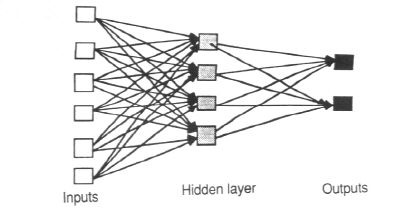
\includegraphics[width=0.60\columnwidth]{images/rna.jpg}%
		\caption{Un simple réseau de neurones}%
	\end{center}
\end{figure}

Le type de réseau de neurones artificiel le plus commun est composé de trois groupes, ou couches, d’unités : une couche d’unités dites « d’entrée » qui est connectée à une couche d’unités « cachées », qui elle-même est connectée à la couche d’unités de « sortie ».

\begin{itemize}
	\item L’activité des unités d’entrée représente l’information brute transmise au réseau.
	\item L’activité des unités cachées est déterminée par celle des unités d’entrée et des connections pondérées entre les unités d’entrée et celles cachées.
	\item Le comportement des unités de sortie dépend de l’activité des unités cachées et des liaisons pondérées entre les unités cachées et celles de sortie.
\end{itemize}

Ce type simpliste de réseau de neurones est intéressant car les unités cachées sont libres de construire leur propre représentation de leurs entrées. Ces poids entre les unités cachées et les unités d’entrée déterminent la valeur d’activité d’une unité cachée, et donc en modifiant ces valeurs, une unité cachée peut choisir ce qu’elle représente.

On peut distinguer les architectures monocouche ou multicouche. Les organisations monocouches, dans lesquelles toutes les unités sont connectées aux autres, constituent le cas le plus général et un plus grand potentiel de puissance de calcul que les organisations multicouches structurées par hiérarchie. Dans les réseaux multicouches, les unités sont numérotées par couche au lieu de suivre une numérotation globale.

Il existe plusieurs stratégies d’apprentissage pour un réseau de neurones artificiel :
\begin{itemize}
	\item \textbf{L’apprentissage supervisé} : Cette stratégie implique un professeur plus intelligent que le réseau lui-même, qui servira de superviseur pour l’apprentissage du réseau de neurones. Par exemple, dans le cas de la reconnaissance faciale, le professeur connaît déjà les noms des personnes qu’il montre au réseau de neurones. Il peut ainsi comparer les réponses données par le réseau et déterminer si des ajustements sont à faire.
	
	\item \textbf{L’apprentissage non supervisé} : Cette technique est requise lorsqu’il n’existe pas d’exemples d’ensembles de données possédant des réponses connues. Prenons par exemple la recherche d’un motif caché dans un ensemble de données. Une application de cela est le « clustering », c’est-à-dire la division en groupes d’un ensemble d’éléments suivant une disposition inconnue.
		
	\item \textbf{L’apprentissage par renforcement} : Cette stratégie est basée sur l’observation. Prenons par exemple un petit robot circulant à travers un labyrinthe. Si le robot tourne à gauche, il obtient une récompense, s’il tourne à droite il hérite d’un malus. On peut supposer que le robot apprendra avec le temps à tourner à gauche. Son réseau de neurones prend une décision avec une valeur d’entrée (tourner à gauche ou à droite) et observe son environnement (récompense ou malus). Si l’observation est négative, le réseau peut ajuster les valeurs des poids entre les unités du réseau afin d’effectuer un choix différent la prochaine fois. L’apprentissage par renforcement est une technique commune dans le domaine de la robotique.
	Cette capacité qu’a le réseau de neurones à apprendre, à faire des ajustements sur sa propre structure à travers le temps, est ce qui le rend si utile dans le domaine de l’intelligence artificielle.
\end{itemize}

Afin de mieux comprendre comment fonctionne un réseau de neurones artificiel, regardons plus en détail le fonctionnement interne d’un réseau de neurones, appelé le perceptron. Il a été inventé en 1957 par Frank Rosenblatt au laboratoire aéronautique de l’université Cornell. Il s’agit du plus simple réseau de neurones possible car son modèle de calcul se base sur un seul neurone.

Un perceptron est composé de plusieurs points d’entrée, d’un processeur et d’un seul point de sortie.

\begin{figure}[!h]%
	\begin{center} 
		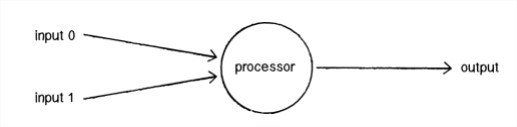
\includegraphics[width=0.60\columnwidth]{images/perceptron.jpg}%
		\caption{Le perceptron}%
	\end{center}
\end{figure}

Un perceptron suit le modèle « feed-forward », ce qui signifie qu’il n’existe aucun cycle au sein du réseau de neurones. Autrement dit les entrées sont envoyés au cœur du neurone qui lui-même transmet ses données à la sortie, comment montré sur le schéma ci-dessus (Figure 4).

Chaque entrée est envoyée au processeur suivant le poids de la liaison qui lui est attribué. Le perceptron calcule ensuite la somme des valeurs qu’il a reçu et à l’aide de sa fonction d’activation choisit quel type de réponse il doit envoyer à l’unité de sortie.

Un perceptron peut bien avoir plusieurs points d’entrée, cependant il reste un neurone seul. Le pouvoir du réseau de neurones réside dans l’interconnexion elle-même. Les perceptrons sont, tristement, plutôt limité dans leur capacités. En lisant un livre sur l’intelligence artificielle on peut y apprendre qu’un perceptron peut seulement résoudre des problèmes dissociables linéairement. Un des exemples les plus simples d’un problème dissociable non-linéairement est le XOR, ou encore « ou exclusif ». Tandis que les opérateurs logiques AND et OR sont des problèmes séparables linéairement, il en est autrement du XOR.

\begin{figure}[!h]%
	\begin{center} 
		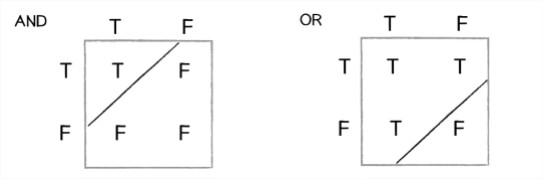
\includegraphics[width=0.60\columnwidth]{images/andor.jpg}%
		\caption{Tables de vérité AND et OR}%
	\end{center}
\end{figure}

Ici il est possible de tirer une ligne afin de séparer les réponses possibles du perceptron.

Le XOR est l’équivalent du OR et du NOT AND. En d’autres termes A XOR B vaut vrai seulement si un seul des deux vaut vrai.

\begin{figure}[!h]%
	\begin{center} 
		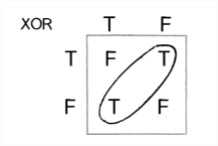
\includegraphics[width=0.30\columnwidth]{images/xor.jpg}%
		\caption{Tables de vérité XOR}%
	\end{center}
\end{figure}

Le problème représenté ci-dessus n’est pas séparable linéairement. En effet, il est impossible de séparer les deux types de sorties par une simple ligne droite.

Nous venons de voir qu’il était impossible pour un perceptron de résoudre le problème du XOR. Mais il n’est pas impossible pour un réseau de deux perceptrons de résoudre le XOR. Si un perceptron résout le OR et qu’un autre se charge du NOT AND alors les deux perceptrons combinés peuvent venir à bout du XOR.

\newpage
\begin{figure}[!h]%
	\begin{center} 
		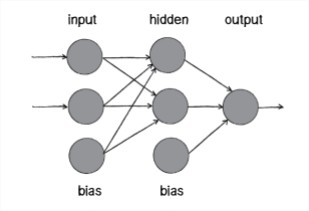
\includegraphics[width=0.60\columnwidth]{images/perceptronmulticouche.jpg}%
		\caption{Un perceptron multicouche}%
	\end{center}
\end{figure}

Entraîner ce genre de perceptrons (Figure 7) est beaucoup plus compliqué. Avec un simple perceptron, il était facile d’évaluer la manière de changer les poids suivant l’erreur obtenue. Mais ici, il y a tellement de connexions différentes entre les neurones qu’il en devient difficile de déterminer l’influence qu’on les neurones entre eux.

Cependant il existe une solution pour optimiser les poids d’un réseau de neurones multicouches qui est connue sous le nom de rétropropagation du gradient (ou backpropagation en anglais). La sortie du réseau est générée de la même manière qu’un perceptron. La différence ici est que les données passent par une couche supplémentaire de neurones avant d’atteindre la sortie. Entraîner le réseau (c’est-à-dire ajuster les poids) implique aussi de prendre en compte l’erreur (la différence entre le résultat désiré et la supposition). L’erreur, néanmoins doit être retransmise à travers tout le réseau. La dernière erreur ajuste en fin de compte le poids de toutes les connexions.

Actuellement il est courant d’utiliser les réseaux de neurones dans le domaine de l’intelligence artificielle. Mais qu’en est-il de l’intelligence artificielle (IA) dans les jeux vidéo ?

TODO Utilisation des RN dans un jeu vidéo pour de l’IA. (Parler de rtNEAT)

\newpage
\subsubsection{Les arbres de comportement}

Dans le domaine des jeux vidéo, il est important de développer des agents dotés d’une intelligence artificielle qui puissent interagir avec l’environnement ou même avec d’autres agents. Dans les jeux un agent peut être un objet, une créature, une personne ou même un système agissant dans le monde virtuel. Suivant le genre, les mécaniques ou le but du jeu, les agents virtuels peuvent être bénéfique pour plusieurs raisons, telles que :

\begin{itemize}
	\item Fournir des ennemis et des alliés au joueur, et donc créer du contenu au jeu.
	\item Créer des entités intelligentes qui viennent compléter le monde virtuel, rendant ainsi l’expérience du joueur plus immersive.
	\item Créer des personnages capables de capter l’empathie du joueur.
\end{itemize}

En général les agents virtuels peuvent interagir avec les humains (sous forme d’avatar dans le jeu) ou avec d’autres agents artificiels. Les agents autonomes intelligents dans les jeux sont appelés PNJ (Personnage Non Joueur) et possèdent des organes sensoriels ou des mécanismes d’actions particuliers à leur but mais aussi à l’environnement qui les entoure. Un PNJ peut, par exemple, être un vendeur de potion humain restant figé dans la ville, attendant que le joueur vienne lui cliquer dessus, ou alors incarner le compagnon du joueur principal, le suivant ainsi durant toutes ses aventures.

Pour développer des agents intelligents, il est nécessaire de construire un vaste répertoire de comportements. Un comportement implique le contrôle de plusieurs actions à travers le temps. Par exemple, imaginez un jeu d’action où les PNJ ont un comportement d’auto-protection. Pour accomplir ce comportement, le PNJ doit vérifier s’il est en danger (par exemple, si sa vie est basse), si c’est confirmé, le PNJ devra alors s’éloigner du joueur. Le nombre de comportements qu’un agent peut utiliser indique le nombre de situations différentes qu’il peut reconnaître et dont il peut agir en conséquence.

Il est aussi important que la méthode utiliser pour contrôler les agents permette une coordination efficace des comportements, afin qu’un agent puisse accomplir son but efficacement, c’est-à-diresans effectuer d’actions aléatoires, inutiles ou stupides (dans un combat, un PNJ ne peut pas s’arrêter pour vendre des objets).

Les agents intelligents possédant des larges répertoires de comportement efficace rendent l’expérience interactive avec l’humain plus intéressante. De plus, dans les jeux vidéo, ces agents ne frustrent pas le joueur, lui permettant une meilleure immersion dans le jeu. Cependant ces résultats ont un coup en terme de complexité tels que :

\begin{itemize}
	\item \textbf{La vitesse} : Beaucoup de comportements implique une forte consommation de la mémoire pour les conserver et une forte utilisation du processeur pour les exécuter. Cependant dans les jeux, rare est la place faite à la partie IA dans la répartition de l’utilisation mémoire/processeur, bien souvent au profit du rendu graphique.
	\item \textbf{La transparence et la fiabilité} : Les développeurs doivent avoir un contrôle total sur les actions de leurs agents. Il ou elle doit être capable de déboguer et de savoir, de manière relativement simple, l’état interne de l’agent, en étant capable de prédire approximativement ses prochaines actions. Ce besoin est particulièrement important pour des raisons de sécurité. Perdre le contrôle de ce que l’agent fait et du moment où il doit le faire peut causer des soucis. En effet, des agents sans contrôle peuvent ruiner l’expérience de jeu. Par conséquent, la quantité de comportements peut rendre le développement plus compliqué et résulter en un système peu fiable.
\end{itemize}

\begin{figure}[!h]%
	\begin{center} 
		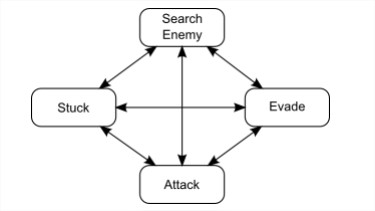
\includegraphics[width=0.60\columnwidth]{images/fsm.jpg}%
		\caption{Une machine à états finis}%
	\end{center}
\end{figure}

\newpage

L’arbre de comportement est venu remplacer la machine à états finis dans le domaine du jeu vidéo en apportant plusieurs avantages :

\begin{itemize}
	\item \textbf{La maintenabilité} : les transitions de l’arbre de décision sont définies dans sa structure, et non par les conditions à l’intérieur des états. Grâce à cela, les nœuds peuvent être conçus indépendamment les uns des autres, ainsi, lorsqu’on ajoute ou retire de nouveaux nœuds (ou même des sous arbres) dans un petite partie de l’arbre, il n’est pas nécessaire de changer les autres parties du modèle.
	\item \textbf{La « scalabilité »}: Lorsqu’un arbre de comportement possède beaucoup de nœuds, il est possible de le décomposer en petits sous arbres, préservant ainsi la lisibilité du modèle graphique.
	\item \textbf{La réutilisabilité} : Grâce à l’indépendance des nœuds dans l’arbre de comportement, les sous arbres sont eux aussi indépendants. Cela permet la réutilisation des nœuds ou des sous arbres à travers d’autres arbres ou projets.
	\item \textbf{La spécialisation} : Bien que les nœuds de l’arbre soient indépendants, ils restent reliés à cause de la structure de l’arbre. Ceci permet au concepteur de construire des sous arbres spécifiques à une tâche sans perdre la flexibilité de son modèle.
	\item \textbf{La parallélisation} : Les arbres de comportements peuvent spécifier des nœuds parallèles qui exécuteront leurs enfants au même instant sans perdre le contrôle du modèle d’exécution. Cela est possible car la parallélisation est contenue localement au nœud parallèle.
\end{itemize}

\newpage
\subsection{Dynamic Game Difficulty Balancing}

Dans beaucoup de jeux d’aujourd’hui, afin de toucher un public plus large allant du casual gamer au hardcore gamer, la possibilité est donnée au joueur de choisir une difficulté au début du jeu. Toutefois, si la courbe de difficulté augmente trop vite pour le joueur, il peut éprouver de la frustration et rester bloqué, tandis que si la difficulté augmente trop lentement, le joueur peut s’ennuyer face à un jeu trop facile.

Même s’il est possible dans certains jeux de modifier la difficulté en cours de jeu, peu de joueurs l’utilisent, par fierté, et finissent soit par se débloquer après une session de jeu peu agréable, soit par abandonner devant un jeu qu’ils trouvent injuste.

C’est pour résoudre ce problème que des jeux utilisent le Dynamic Game Difficulty Balancing\cite{hunicke2005case}. C’est une technique qui permet de changer dynamiquement certains éléments (comportement de PNJ, paramètres, etc ...) au cours du jeu, pour mieux s’adapter au niveau de compétence du joueur, ou même (plus rarement) à son style de jeu. Son but est donc de moduler la difficulté, afin que le jeu représente un challenge intéressant du début à la fin et de garder le joueur dans ce que l'on appelle le flow (état dans lequel le joueur est concentré sur le jeu et ne voit pas le temps passer).

\begin{figure}[!h]%
	\begin{center} 
		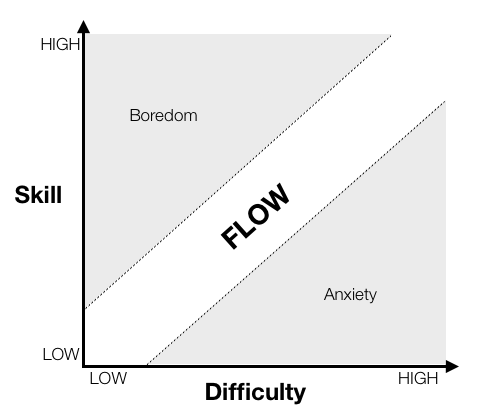
\includegraphics[width=0.60\columnwidth]{images/flow.png}%
		\caption{Représentation de la zone de flow}%
	\end{center}
\end{figure}

\newpage
S’il existe presque autant d’approches différentes à cette technique que de jeux qui l’utilisent, il faut néanmoins dans tous les cas régulièrement déterminer et analyser les performances du joueur au moyen d’une fonction heuristique, qui fournit rapidement un résultat concret, même si pas optimal (très utilisé pour les jeux, dans lesquels les performances sont critiques).

De plus, des études ont montré qu’une fonction heuristique déterminée à l’aide d’un réseau de neurones artificiels (ANN) donne de meilleurs résultats qu’une fonction heuristique faite par des humains.
Il est ainsi possible, afin de moduler le comportement des PNJ, de pondérer la probabilité de ses actions en fonction des performances du joueur.

Par exemple, dans un jeu de tir à la première personne (FPS), le jeu pourra prendre en compte :

\begin{itemize}
	\item Le nombre de points de vie actuel du joueur
	\item Le nombre de munitions actuel du joueur
	\item La précision du joueur (pourcentage de tirs qui touchent une cible)
	\item Durée de vie moyenne d’un ennemi
	\item etc ...
\end{itemize}

Et à partir de ces informations, en fonction de comment le joueur se débrouille, le jeu pourra décider de :

\begin{itemize}
	\item Faire apparaître plus ou moins d’ennemis
	\item Rendre les ennemis plus ou moins résistants et/ou intelligents
	\item Faire apparaître plus ou moins de caisses de munitions et/ou kits de santé
	\item etc ...
\end{itemize}

Toutefois, cette méthode a tout de même quelques inconvénients. Si les joueurs sont au courant de l'existence de cette méthode dans le jeu, ils peuvent en tirer profit, par exemple en faisant exprès de mal jouer avant une rencontre avec un boss pour le rendre plus simple. Il est donc possible que des jeux utilisent ce système mais ne le mentionnent pas afin d'éviter les abus. De plus, à cause des nombreuses problématiques de game design que cela soulève, le nombre de jeux qui utilisent cette technique est assez restreint.

\newpage
\subsubsection{Resident Evil 5}

Dans Resident Evil 5 (2009), il est possible de sélectionner une difficulté de départ, mais celle-ci n’est pas fixe. Pendant le jeu, un système appelé « Difficulty Scale » analyse et note la performance du joueur sur une échelle de 1 à 10 et adapte la difficulté du jeu en modifiant certains paramètres comme :

\begin{itemize}
	\item La résistance et les dommages des ennemis.
	\item Le comportement et panel d'attaque des ennemis.
\end{itemize}

Le tableau ci-dessous indique les notes associés aux différentes actions du joueur :

\begin{center} 
	\begin{tabular}{|l|r|}
		\hline
		Action 									&Points associés\\
		\hline
		Mort du joueur							&-1200\\
		Joueur proche de la mort				&-650\\
		Subit des dégats lourds					&-500\\
		Subit des dégats légers					&-400\\
		\hline
		Touche un ennemi						&+2\\
		Touche un ennemi à un endroit sensible	&+30\\
		Évite une attaque						&+45\\
		Tue un ennemi							&+80\\
		Fait un coup critique					&+100\\
		\hline
	\end{tabular}
\end{center}

Ici, la difficulté choisie au départ sert de bornes pour la difficulté dynamique. Ainsi, si le joueur choisit la difficulté minimale, même s’il se débrouille très bien par la suite, la difficulté dynamique ne pourra pas dépasser un certain seuil. Et inversement si le joueur choisit une difficulté initiale élevée, et que par la suite ne fait que mourir, la difficulté ne pourra pas baisser en dessous d’un certain niveau.

\newpage
\subsubsection{La série Mario Kart : objets et PNJ}

Mario Kart est un jeu de course dans lequel le joueur peut obtenir des objets pour l'aider en roulant sur un cube. Ces cubes donnent un objet aléatoire, mais dépendant de la position du joueur dans la course. Ainsi, si le joueur est bien placé, il aura des chances augmentées de recevoir des objets considérées « faibles », comme une banane ou une carapace verte, tandis que si le joueur se retrouve à la fin du classement, ce sont ses chances de recevoir des objets considérées « fortes », comme la fameuse tortue bleue qui augmentent.

 Le tableau ci-dessous représente les probabilités d'obtenir un objet en fonction de la position dans la course dans Mario Kart 64.

\begin{center} 
	\begin{tabular}{|l|c|c|c|c|c|c|c|c|}
		\hline
		Capacité 				&1\ier{}&2\up{e}&3\up{e}&4\up{e}&5\up{e}&6\up{e}&7\up{e}&8\up{e}\\
		\hline
		Banane (1)				&30\%	&		&		&		&		&		&		&		\\
		Bananes (5)				&5\%	&5\%	&		&		&		&		&		&		\\
		Caparace verte (1)		&30\%	&5\%	&		&		&		&		&		&		\\
		Carapaces vertes (3)	&5\%	&10\%	&10\%	&		&		&		&		&		\\
		Caparace rouge (1)		&5\%	&15\%	&20\%	&15\%	&10\%	&		&		&		\\
		Caparaces rouges (3)	&		&20\%	&20\%	&20\%	&20\%	&20\%	&20\%	&20\%	\\
		Carapace bleue			&		&		&		&5\%	&5\%	&10\%	&10\%	&15\%	\\
		Éclair 					&		&5\%	&5\%	&10\%	&10\%	&15\%	&20\%	&20\%	\\
		Fausse boîte à objets	&10\%	&5\%	&		&		&		&		&		&		\\
		Étoile 					&		&5\%	&10\%	&15\%	&15\%	&20\%	&30\%	&30\%	\\
		Boo						&5\%	&5		&		&		&		&		&		&		\\
		Champignon Turbo (1)	&10\%	&5\%	&5\%	&5\%	&5\%	&		&		&		\\
		Champignons Turbo (3)	&		&15\%	&20\%	&20\%	&25\%	&25\%	&10\%	&5\%	\\
		Champignon Turbo doré	&		&5\%	&10\%	&10\%	&10\%	&10\%	&10\%	&10\%	\\
		\hline
	\end{tabular}
\end{center}

Les PNJ ont également droit à ces probabilités modifiées, mais ont en plus un comportement qui s’adapte en fonction de leur classement. En effet, un PNJ en tête de classement verra sa vitesse maximum  réduite et sera moins agressif, tandis qu’un PNJ en bas du classement aura une vitesse maximum augmentée et deviendra plus agressif.

Malheureusement cette dernière technique provoque un effet nommé « rubber band effect » (« effet élastique »), car le joueur peut avoir l’impression que tous les autres PNJ sont liés à lui par un élastique, puisqu’ils ne peuvent pas prendre trop d’avance ou trop de retard par rapport à lui.

\newpage
\subsubsection{Left 4 Dead et son AI Director}

Le meilleur exemple actuel (connu) pour ce type d’IA se trouve du côté de Valve, et plus précisément dans leur survival horror FPS, Left 4 Dead (2008). Dans celui ci, un groupe de quatre joueurs doit se frayer un chemin dans un niveau infesté de zombies en tout genre.

Cette intelligence artificielle, surnommée « \textbf{\textit{AI Director}} »\cite{aidirector} (que nous appellerons simplement par la suite « \textit{Director} ») analyse constamment les performances des joueurs afin de proposer une expérience plus intéressante. Mais il ne se contente pas d’analyser les performances individuelles, il analyse également la performance collective du groupe.

\begin{figure}[!h]%
	\begin{center} 
		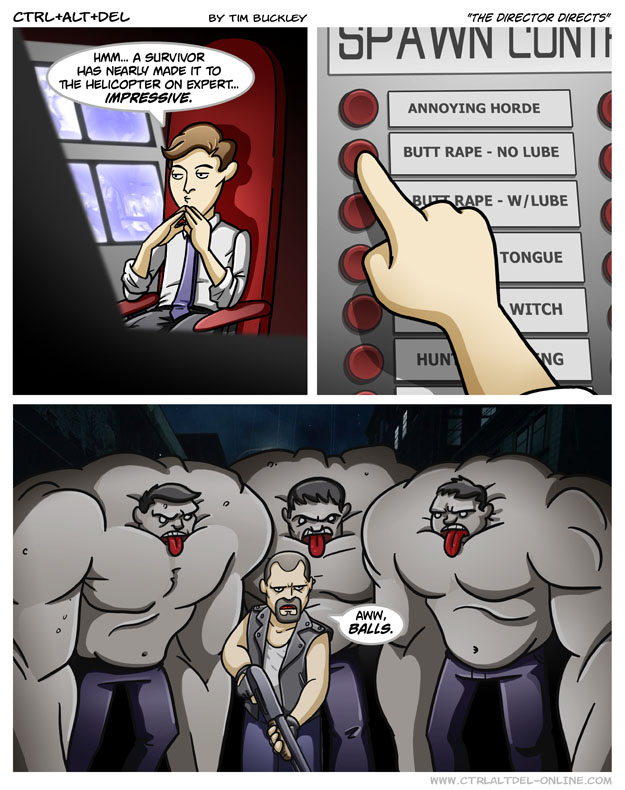
\includegraphics[width=0.60\columnwidth]{images/aiDirector.png}%
		\caption{The Director Directs, de Tim Buckley}%
	\end{center}
\end{figure}

Le \textit{Director} suit un cycle tout au long de la partie. Dés que les joueurs sortent de la zone de départ, l’étape de « Build Up » commence. Pendant cette étape, un nombre relativement constant d'ennemis attaque les joueurs. Lorsque le niveau d’intensité du groupe (pression calculée pour chaque joueur, augmente plus les ennemis sont proches) atteint un certain seuil, l’étape de « Peak » est enclenchée et plus aucun ennemi ne spawn. L’étape de « Relax » prend alors le relais pendant environ 30 secondes, durant lesquelles les joueurs peuvent se soigner et récupérer, après quoi le processus recommence, et ce jusqu’à la fin du niveau.

La fonction principale du \textit{Director} est de s’occuper de l’apparition et du placement des ennemis. Il y a deux catégories d’ennemis, les ennemis communs et les boss. Pour les ennemis communs, il peut décider de placer des ennemis devant les joueurs, qui errent sans but et attaquent les joueurs à vue, ou les placer sur les côtés et derrière les joueurs, et ceux-ci foncent directement vers les joueurs, même s’ils ne sont pas en vue.

Pour ce qui est des boss, ils attaquent à vue également, mais le il ne peut les faire apparaître qu’à certains endroits spécifiques de la carte, le long du chemin principal. En revanche, si les joueurs essayent de les éviter en passant par un chemin parallèle, le \textit{Director} s’en rendra compte et rendra le boss agressif, qui ira attaquer les joueurs.

\begin{figure}[!h]%
	\begin{center} 
		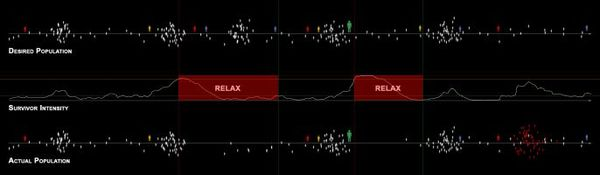
\includegraphics[width=1.0\columnwidth]{images/aiDirector.jpg}%
		\caption{Exemple d'actions du \textit{Director}}%
	\end{center}
\end{figure}

Dans la figure ci-dessus, qui représente le parcours d'un niveau, la barre du haut représente les ennemis que le \textit{Director} a placé lors de la génération du niveau, tandis que la barre du bas représente la présence réelle des ennemis. On peut remarquer que lorsque le niveau d'intensité des joueurs, représenté par la barre du milieu, atteint un certain seuil, l'étape de « Relax » est enclenchée, ce qui fait disparaître les ennemis. À l'inverse, si le niveau d'intensité devient trop bas, le \textit{Director} fait apparaître de nouveaux ennemis.

\newpage
De plus, le \textit{Director} ne se contente pas de modifier les éléments du gameplay, c’est également lui qui gère les répliques lancées par les personnages, modifie dynamiquement la musique pour s’adapter au moment, ainsi que la position des objets récupérables par les joueurs. Il est aussi responsable de certains effets sonores et visuels, qu’il peut décider d’ajouter pour amplifier la tension.

le \textit{Director} de Left 4 Dead 2 est même capable de modifier dynamiquement l’agencement du niveau et donc de modifier le chemin que les joueurs doivent suivre.

Malheureusement, son existence et son fonctionnement étant connu par les joueurs, ceux-ci n’hésitent pas à en tirer profit pour rendre certaines parties du jeu plus simple en faisant exprès de mal jouer pour réduire la difficulté à certains moments critiques du jeu.

\begin{figure}[!h]%
	\begin{center} 
		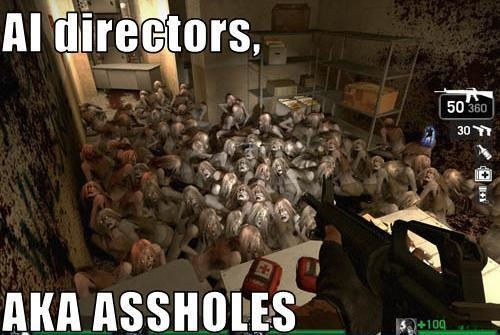
\includegraphics[width=0.80\columnwidth]{images/aiDirector2.jpg}%
		\caption{Le \textit{Director} est parfois méchant}%
	\end{center}
\end{figure}

%\newpage
%\subsection{Cheating / Procedural / Data mining}

\newpage
\subsection{General Video Game Playing, l'IA qui apprend à jouer}

Bientôt, il n’y aura plus du tout besoin d’humains dans la boucle de création et consommation de jeu.

Si les IA capables de jouer à des jeux de société existent depuis longtemps, celles-ci étaient limitées et ne pouvaient jouer qu’à un seul jeu. Ce n’est pas le cas des IA suivant la technique de GGP (\textbf{G}eneral \textbf{G}ame \textbf{P}laying), et son homologue pour les jeux vidéo, la technique de GVGP\cite{levine_et_al:DFU:2013:4337} (\textbf{G}eneral \textbf{V}ideo \textbf{G}ame \textbf{P}laying).

Grâce à ce type d'IA, il serait possible de réduire la quantité de tests à effectuer par des humains sur le jeu pour découvrir les bugs de haut niveau. Par exemple, détecter les failles de gameplay avant les joueurs pour éviter les abus, ou vérifier si un monde généré procéduralement est jouable par des humains.

Une autre application, à plus long terme, serait d'éviter aux développeurs d'avoir à adapter, voir réécrire, une IA pour chaque jeu. En effet, une IA suffisamment autonome avec un large champ d'apprentissage devrait être capable d'apprendre seule à jouer à n'importe quel type de jeu, dans le rôle de n'importe quel PNJ, réduisant considérablement le temps de développement d'un jeu.

\begin{figure}[!h]%
	\begin{center} 
		
\includegraphics[width=0.60\columnwidth]{images/robotplaying.jpg}%
		\caption{Le joueur du futur}%
	\end{center}
\end{figure}

\newpage
Ce domaine a gagné en popularité ces dernières années, notamment grâce à une IA de GVGP qui a gagné le prix du public de la compétition annuelle 2015\cite{mariolives} de GGP organisée par l’AAAI (\textbf{A}ssociation for the \textbf{A}dvancement of \textbf{A}rticifial \textbf{I}ntelligence).

Cette IA est notamment capable d’apprendre à jouer à un niveau de Mario, un jeu de plateforme 2D, de s’adapter aux différents obstacles qui le composent, et même d’apprendre certaines mécaniques (sauter sur un Koopa pour le tuer).

\begin{figure}[!h]%
	\begin{center} 
		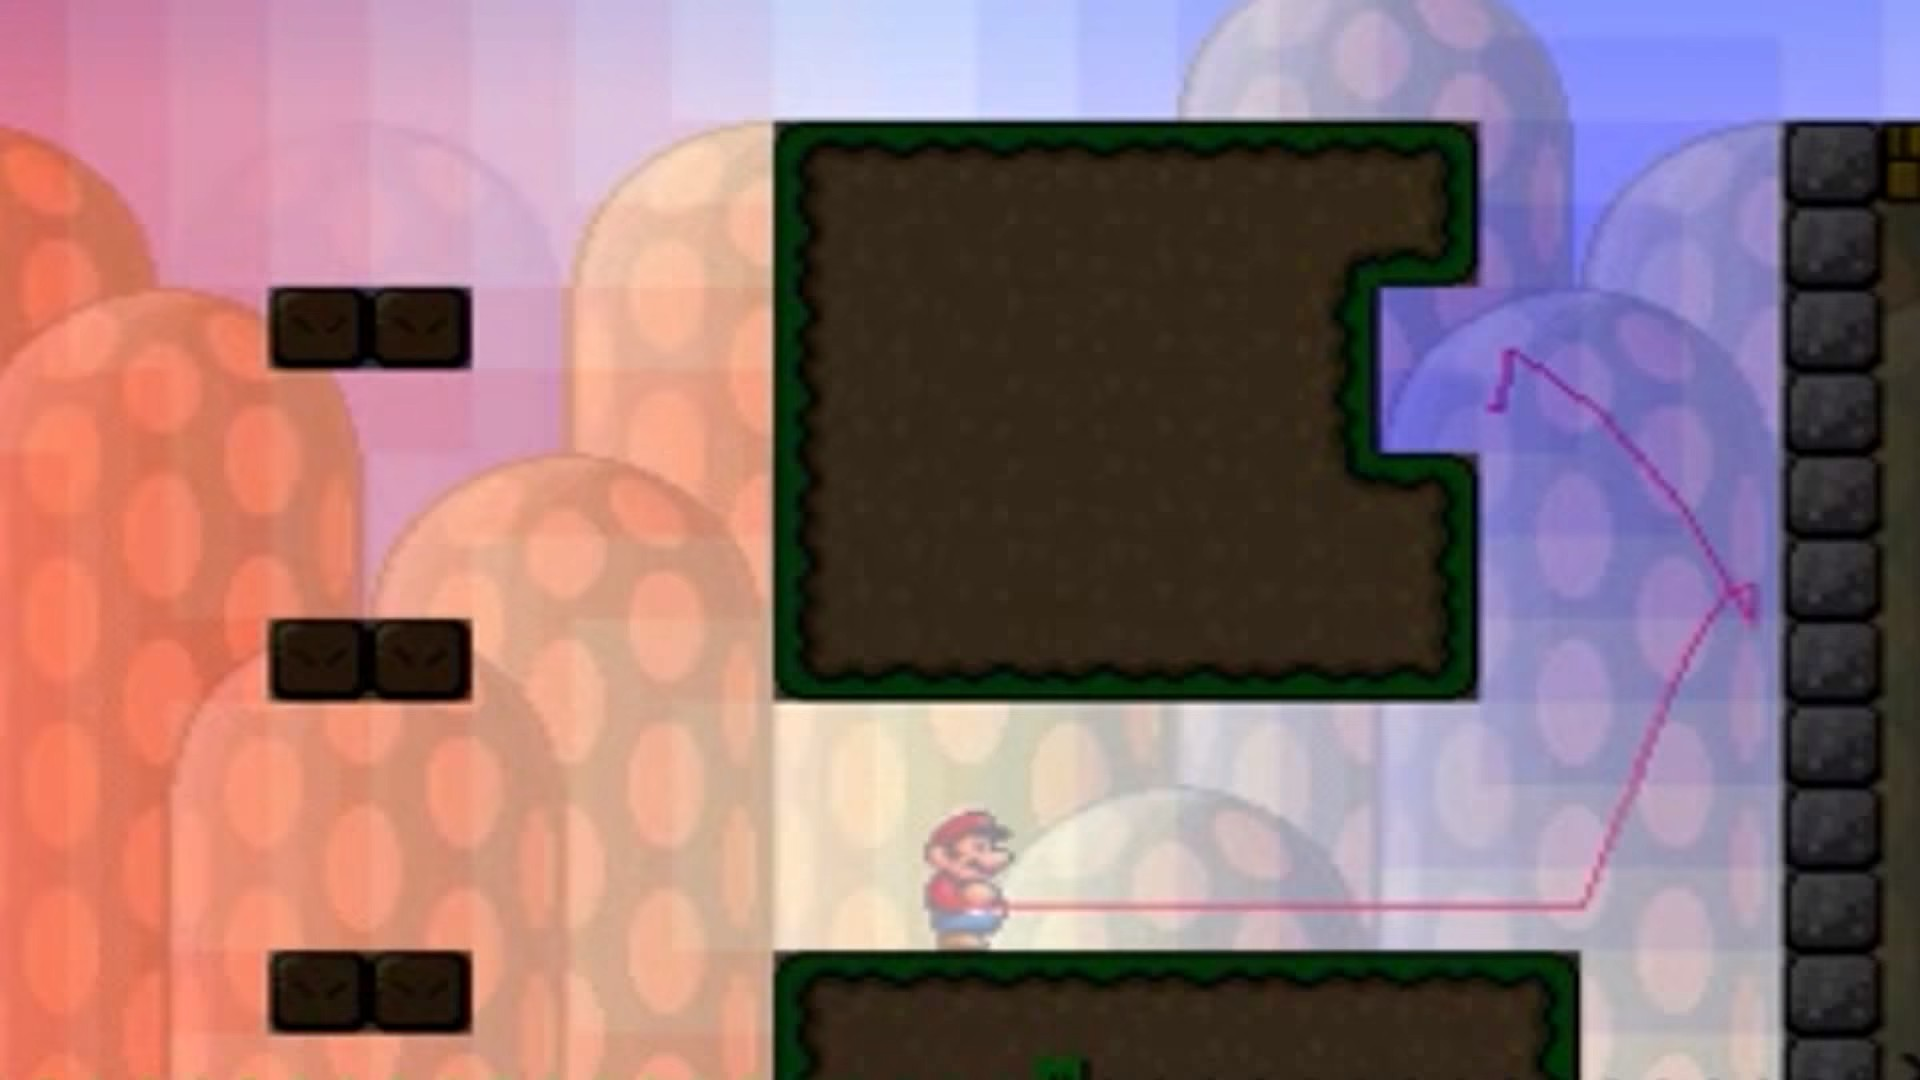
\includegraphics[width=0.60\columnwidth]{images/mario.jpg}%
		\caption{Prédiction de déplacement de l'IA}%
	\end{center}
\end{figure}

Un autre point intéréssant de cette IA est qu'elle est (relativement) consciente d'exister. Elle dispose ainsi de plusieurs émotions (la peur, la satisfaction, la curiosité et la faim) qui conditionnent son comportement. Par exemple, si son niveau de curiosité est élevé, elle essayera d'interagir avec les éléments de son environnement, tandis que ramasser des pièces augmentera sa satisfaction. Il est également possible d'interagir avec cette IA et de lui poser des questions ou de lui donner des informations sur le jeu. 

\newpage
\subsection{Des jeux par les IA}

Comme nous l'avons vu dans la partie précédente, l'époque où il n'y avait que les humains qui jouaient aux jeux vidéo est révolue, dorénavant, même les IA apprennent à y jouer.

Mais une autre époque pourrait également bientôt se finir. En effet, depuis quelques années, d'autres projets d'IA ont vu le jour, non pas pour jouer aux jeux vidéo, mais pour les créer. 

Ces programmes ne demandent qu'une description sommaire mais livrent un jeu jouable.

\begin{figure}[!h]%
	\begin{center} 
		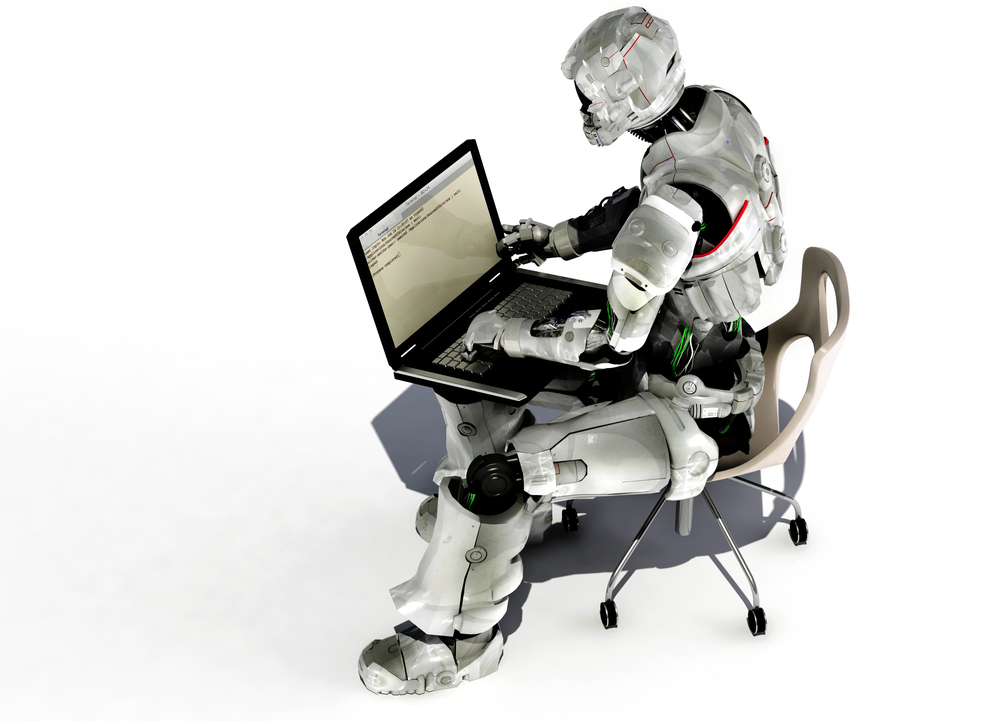
\includegraphics[width=0.60\columnwidth]{images/robotdeveloping.jpg}%
		\caption{Robot développant un jeu (fiction)}%
	\end{center}
\end{figure}

\newpage
\subsubsection{Video Game Description Language}

Le \textbf{V}ideo \textbf{G}ame \textbf{D}escription \textbf{L}anguage\cite{schaul2013video} (VGDL) est un langage imaginé et implémenté par Tom Schaul, qui permet de générer un jeu vidéo en 2D en quelques dizaines de lignes de codes.

Dans un premier temps, il faut fournir au programme un fichier texte, divisé en quatre sections, chacune décrivant un aspect du jeu :

\begin{itemize}
	\item \textbf{LevelMapping} : dans cette section est expliquée comment transformer le fichier de description de niveau en niveau.
	\item \textbf{SpriteSet} : dans cette section sont définies toutes les entités visibles que le jeu utilisera (supporte l'héritage).
	\item \textbf{InteractionSet} : dans cette section sont définies les actions à effectuer lorsque deux sprites entrent en collision.
	\item \textbf{TerminationSet} : dans cette section sont définies les conditions de victoire ou de défaite.
\end{itemize}

\begin{figure}[!h]%
	\begin{center} 
		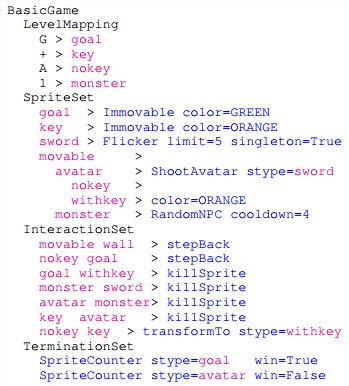
\includegraphics[width=0.60\columnwidth]{images/vgdlgame.jpg}%
		\caption{Example de code pour produire un RPG classique}%
	\end{center}
\end{figure}

\newpage
Il faut ensuite lui fournir un autre fichier texte décrivant le niveau, dans lequel chaque caractère représente une entité.

\begin{figure}[!h]%
	\begin{center} 
		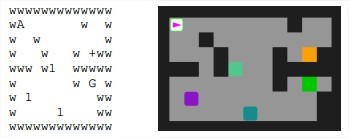
\includegraphics[width=0.60\columnwidth]{images/vgdllevel.jpg}%
		\caption{Exemple de texte pour produire un niveau}%
	\end{center}
\end{figure}

Le but premier de ce langage est de permettre la génération rapide d'une multitude de jeux, qui eux serviront à tester différentes techniques d'apprentissage, pour valider leur généralité.

Le langage étant très jeune, il manque encore de fonctionnalités, mais son développeur a pour objectif d'ajouter le support du multi-joueur, d'améliorer le système de récompense pour faciliter le Reinforcement Learning, ou encore d'ajouter des ressources (vie, mana, etc ...) aux entités.

Malgré cette jeunesse, le langage a déjà permis de reproduire des versions simplifiées de jeux classiques, comme Space Invaders (1978), Pac-Man (1980) ou encore Super Mario Bros (1985). 

\newpage
\subsubsection{ANGELINA}

ANGELINA\cite{cook2014ludus} (\textbf{A} \textbf{N}ovel \textbf{G}ame-\textbf{E}volving \textbf{L}abrat \textbf{I}’ve \textbf{N}amed \textbf{A}NGELINA) est une IA développée par Michael Cook, un chercheur britannique à l’université de Falmouth. Elle peut générer des jeux, avec une ambiance, des graphismes et un gameplay qui respectent (dans une certaine mesure) la description fournie.

Comme pour le VGDL, il faut lui fournir un fichier texte (en YAML, un format de représentation de données avec une grande lisibilité), pour décrire les différentes entités qui composeront le jeu.

\begin{figure}[!h]%
	\begin{center} 
		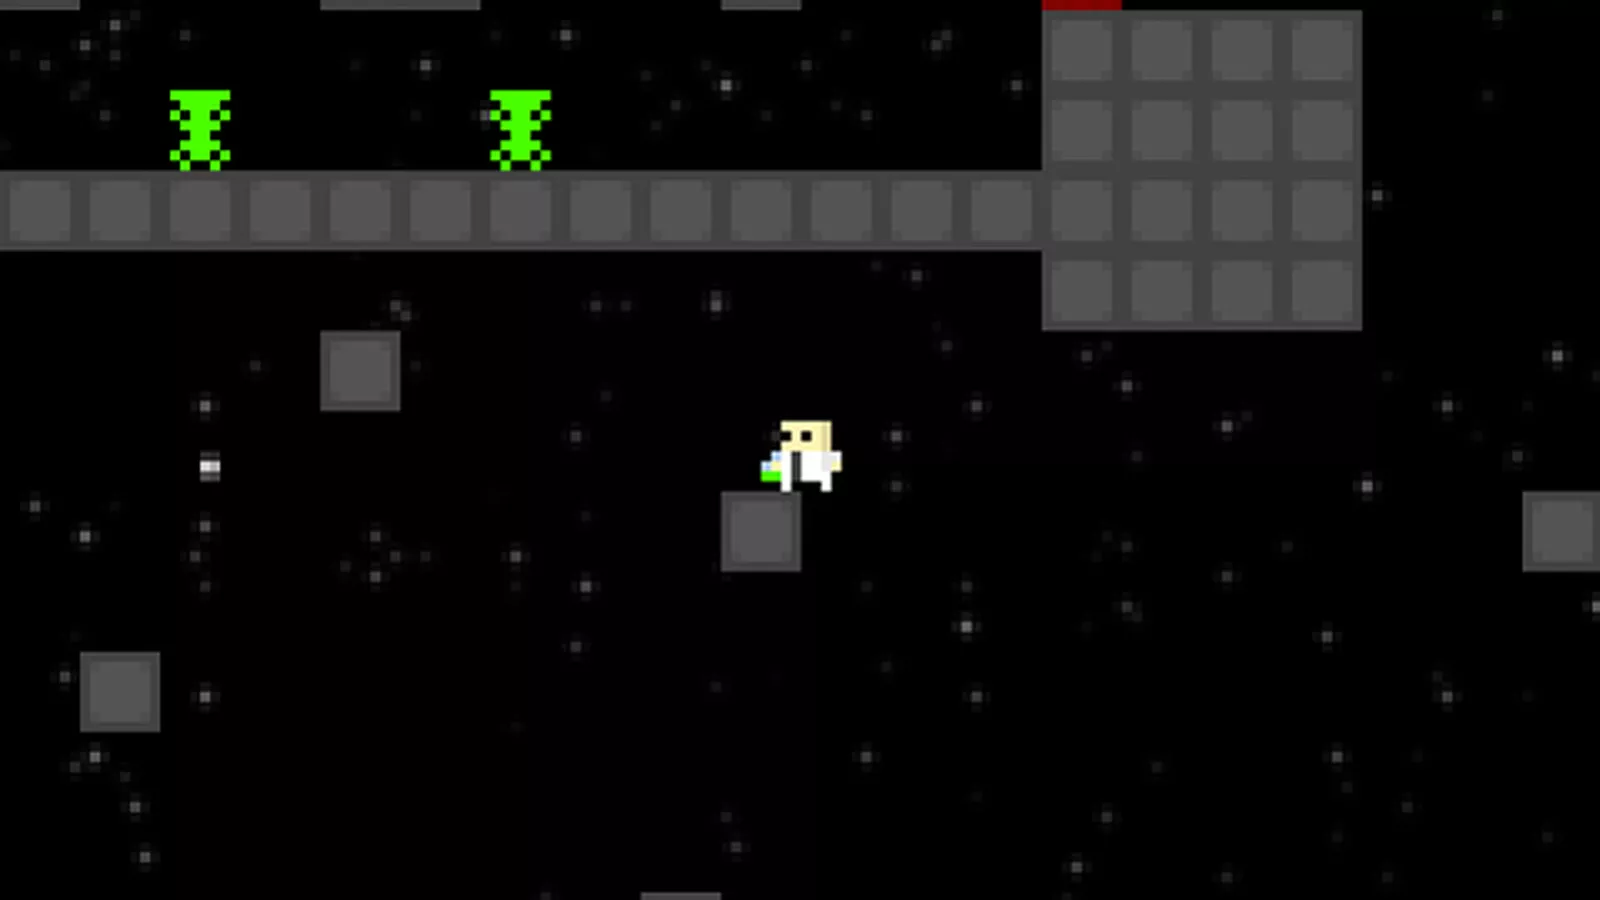
\includegraphics[width=0.60\columnwidth]{images/angelina.png}%
		\caption{Exemple de jeu produit par ANGELINA}%
	\end{center}
\end{figure}

En revanche une des forces d'ANGELINA est qu'elle n'a pas besoin de fichier pour créer un environnement. C'est donc elle qui a la responsabilité de générer un environnement logique et jouable, dans lequel il est possible de se déplacer. Cela implique une analyse poussée des mécaniques du jeu pour définir les zones atteignables par le joueur, et éviter de créer une situation de « Softlock », dans laquelle le joueur ne peut plus progresser.

\newpage
Utilisée lors du Ludum Dare 28, qui avait pour thème « You Only Get One », il s'agit de la première IA à participer à une compétition de game designer. Le but du jeu qu'elle a créé pour cette occasion est de ramasser tous les bateaux présents dans le niveau, en évitant des êtres humanoïdes non identifiés patrouillant dans les salles, le tout dans une ambiance extrêmement glauque. La description du jeu a elle aussi été générée par ANGELINA, suivant un template. 

Toutes les ressources utilisées pour générer le jeu ont été choisies par ANGELINA, qui après avoir analysé le thème, a décidé de faire un jeu à l'ambiance glauque.

\begin{figure}[!h]%
	\begin{center} 
		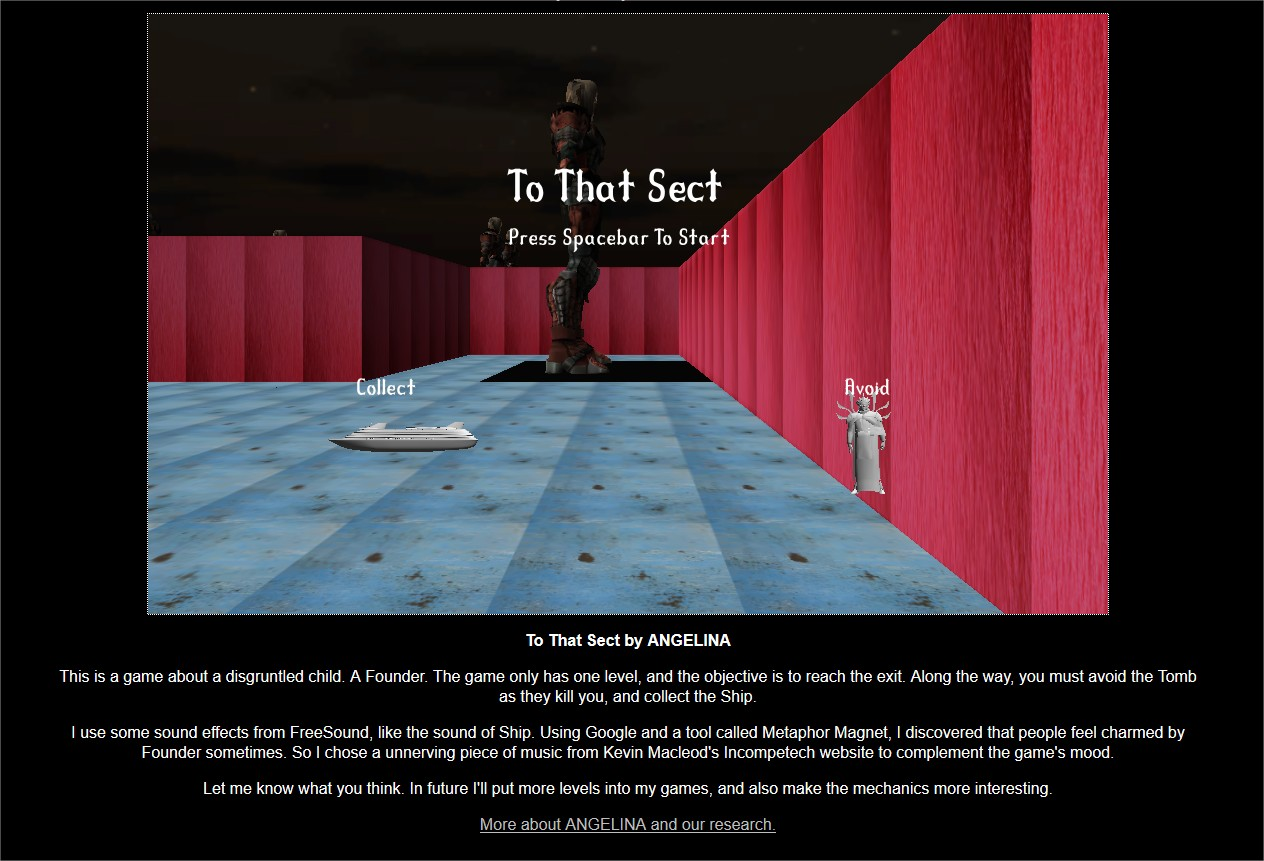
\includegraphics[width=1.0\columnwidth]{images/angelinacreepy.jpg}%
		\caption{Autre jeu produit par ANGELINA}%
	\end{center}
\end{figure}

Lorsque le joueur a récupéré tous les bateaux, un message apparaît sur l'écran pour lui signifier sa victoire, et l'invite à appuyer sur « Echap » pour quitter le jeu, mais l'appui sur cette touche ne fait rien. 

Bug innocent, ou début de quelque chose de plus inquiétant, le développeur d'ANGELINA n'a pas souhaité se prononcer.

De là à dire que Skynet est déjà parmi nous, il n'y qu'un pas. 

%------------------------------------------------

\newpage
\section{De l’importance de l’IA pour l’immersion du joueur}

Dans cette partie, nous parlerons de l’intelligence artificielle qui n’est pas flagrante, mais qui rend, inconsciemment pour le joueur, l'expérience de jeu plus réaliste et immersive. Cette intelligence artificielle est bien plus importante dans les jeux à un seul joueur que dans les jeux multi-joueurs, dans lesquels il est dur de maintenir le joueur dans un univers fictif à cause de la présence d’autres joueurs dont le comportement est difficilement contrôlable et peut être perturbateur.

\begin{figure}[!h]%
	\begin{center} 
		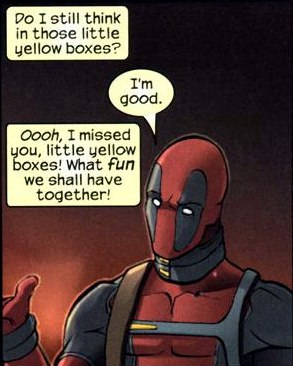
\includegraphics[width=0.60\columnwidth]{images/deadpool.png}%
		\caption{Deadpool, personnage de l’univers Marvel connu pour ne pas beaucoup respecter le 4ème mur}%
	\end{center}
\end{figure}

\newpage

\subsection{Suspension consentie de l'incrédulité}

\begin{wrapfigure}{r}{0.4\textwidth}
	\begin{center}
		
\includegraphics[width=0.40\textwidth]{images/repeat1.png}
	\end{center}
	\caption{Why RPG NPCs Always Repeat Themselves, de Dorkly}
\end{wrapfigure}

Lorsqu’un PNJ répète sans cesse le même dialogue, le joueur est ramené à la réalité. Quand un PNJ rencontre un problème de recherche de chemin et fonce obstinément dans un mur ou n’arrive pas à se déplacer d’un point à un autre, le joueur est ramené, brutalement, à la réalité. 

Ces actions, souvent sans le vouloir, cassent le quatrième mur, et mettent fin à ce que l’on appelle la Suspension Consentie de l’Incrédulité (aussi connue sous le nom de Suspension of disbelief en anglais). Il s’agit d’une sorte de contrat que le joueur signe avec l’œuvre de fiction (que ce soit un jeu, un film, un livre), dans lequel le joueur accepte de mettre de côté son scepticisme le temps de la consultation de l’œuvre en question. 

\begin{figure}[!h]%
	\begin{center} 
		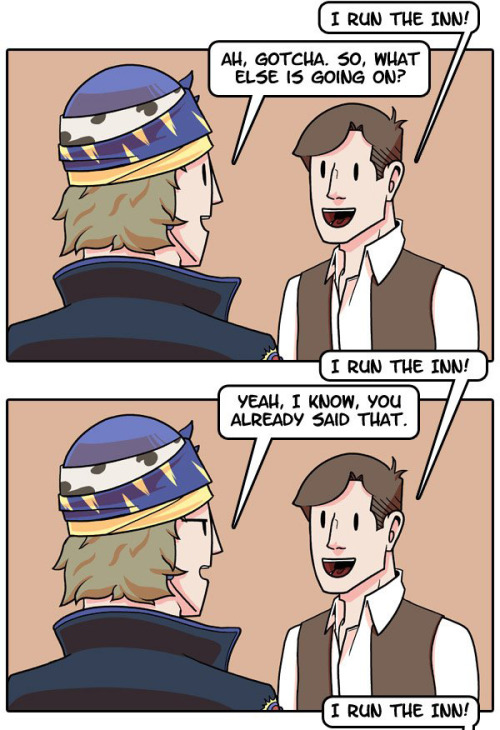
\includegraphics[width=0.40\columnwidth]{images/repeat2.png}%
		\caption{Why RPG NPCs Always Repeat Themselves, de Dorkly}%
	\end{center}
\end{figure}

Il peut ainsi s’immerger dans un univers avec des éléments imaginaires, pour peu que ceux-ci restent crédibles, et que les règles qui régissent l’œuvre restent constantes.
Lorsque ce contrat est rompu (par définition, il ne peut être rompu que par l’œuvre de fiction), il est difficile de faire replonger un joueur dans l’univers du jeu, avec lequel il restera toujours un peu distant, et cela renforce le solipsisme du joueur.

\begin{figure}[!h]%
	\begin{center} 
		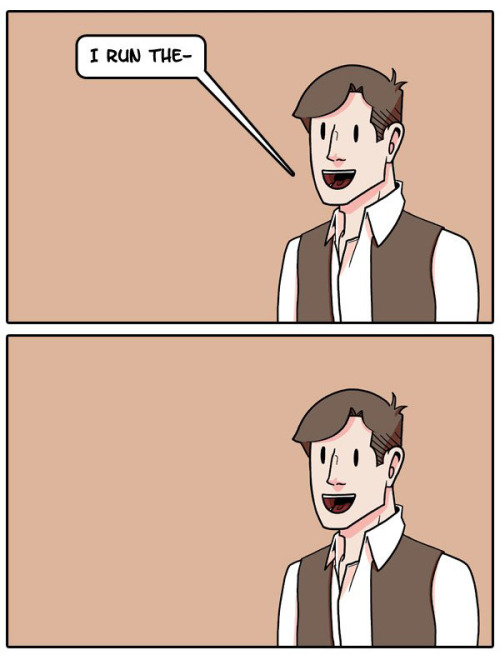
\includegraphics[width=0.40\columnwidth]{images/repeat3.png}%
		\caption{Why RPG NPCs Always Repeat Themselves, de Dorkly}%
	\end{center}
\end{figure}

\newpage
\subsubsection{Solipsisme}

Le solipsisme (du latin \textbf{\textit{solus}}, « seul » et \textbf{\textit{ipse}}, « soi-même ») est une attitude selon laquelle, la seule certitude absolue pour le sujet pensant, est que lui-même existe. Cette attitude est répandue dans la société, et il est tout à fait normal de l’avoir ressenti de façon passagère.

Mais c'est dans les jeux vidéo (principalement ceux à un seul joueur) qu'elle est le plus présente, et qu’on essaie le plus de la faire disparaître. En effet, le but d’un jeu narratif est d’immerger le joueur, et un très bon moyen pour cela est de lui faire oublier qu’il est la seule personne effectivement douée de conscience.

\begin{figure}[!h]%
	\begin{center} 
		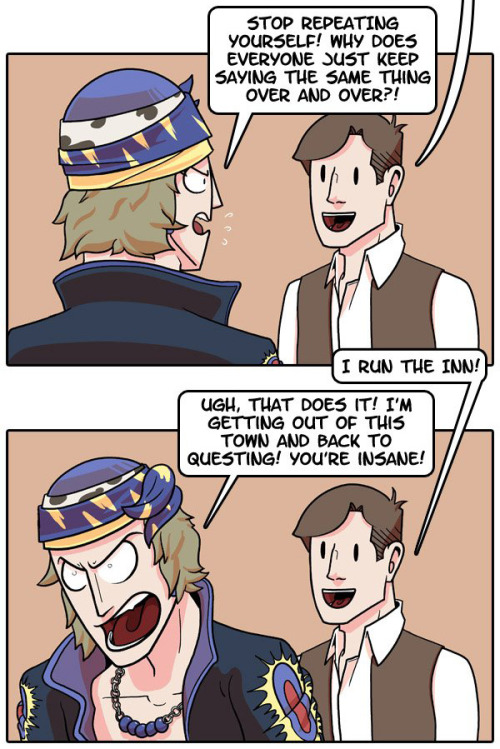
\includegraphics[width=0.40\columnwidth]{images/repeat3.jpg}%
		\caption{Why RPG NPCs Always Repeat Themselves, de Dorkly}%
	\end{center}
\end{figure}

Evoluer dans un monde photoréaliste et crédible est un bon moyen de garder le joueur immergé. Toutefois, rares sont les jeux sans PNJ, il faut donc s’assurer qu’eux aussi ne cassent pas cette immersion. Pour cela, les doter de réactions naturelles est la manière la plus efficace pour arriver à ce résultat.

Ainsi, de de plus en plus de développeurs de MMORPG (Jeu de Rôle Massivement Multijoueur) décident de donner plus de profondeur aux PNJ (amicaux comme ennemis).

\newpage
C’est le cas notamment dans EverQuest Next (en cours de développement), dans lequel chaque PNJ se voit attribuer certains traits de caractère, ce qui affecte la façon dont il interagit avec les joueurs, ainsi qu’avec les autres PNJ. 

De plus, toujours dans EverQuest Next, les monstres ne sont pas regroupés en « camps de monstres », dans lesquels ils ne font qu’attendre, immobiles et apathiques, qu’un joueur vienne les sortir de leur léthargie, comme c’est le cas dans beaucoup de MMORPG actuels. 

A la place, un monstre pourra former un groupe avec d’autres monstres et tendre des embuscades sur une route, et ils pourront décider de  partir vers d’autres horizons s’ils jugent que cette zone n’est pas assez fructueuse, ou se faire chasser par des joueurs s'ils restent au même endroit trop longtemps.

Toutefois, si le réalisme des PNJ androïdes n’arrive pas à la hauteur des attentes du joueur, celui-ci peut être confronté à ce que l'on appelle la vallée dérangeante (plus connue sous son nom anglais d’uncanny valley).

\begin{figure}[!h]%
	\begin{center} 
		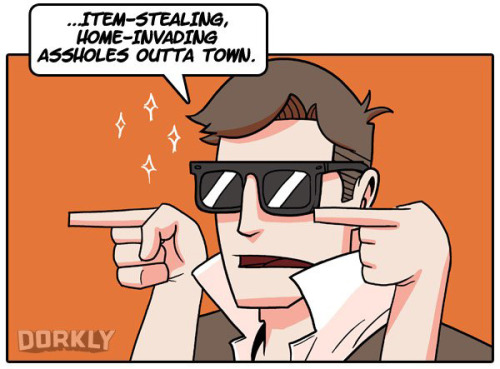
\includegraphics[width=0.60\columnwidth]{images/repeat4.png}%
		\caption{Why RPG NPCs Always Repeat Themselves, de Dorkly}%
	\end{center}
\end{figure}

\newpage
\subsubsection{Vallée dérangeante}

La vallée dérangeante est une théorie selon laquelle plus une créature androïde ressemble à un être humain, plus on remarque ses imperfections, même minimes, et plus elles nous dérangent. Cette théorie a été publiée en 1970 par le roboticien japonais Masahiro Mori, dans le cadre de ses recherches sur les réponses émotionnelles des robots.

\begin{figure}[!h]%
	\begin{center} 
		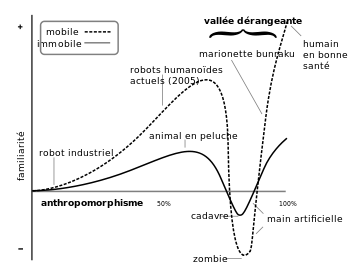
\includegraphics[width=0.60\columnwidth]{images/uncannyValley.png}%
		\caption{Représentation de la vallée dérangeante}%
	\end{center}
\end{figure}

Dans les jeux vidéo, c’est le plus souvent dû au physique (proportions du corps) et à l’animation (principalement du visage) des PNJ androïdes, qui se rapprochent de plus en plus de la perfection, mais dont la moindre imperfection nous paraît grotesque.

%\begin{figure}[!h]%
%	\begin{center} 
%		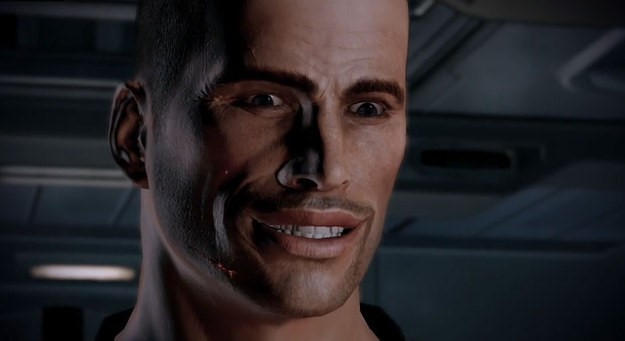
\includegraphics[width=0.60\columnwidth]{images/shepard.jpg}%
%		\caption{Commandant Shepard et son sourire dérangeant, Mass Effect 3, BioWare}%
%	\end{center}
%\end{figure}

Toutefois, leur comportement joue également un rôle très important. Le personnage de Natalya, personnage secondaire de GoldenEye 007 (1997) notamment, est devenu célèbre pour ses piètres capacités intellectuelles. En effet, plusieurs missions le long du jeu requièrent de l’escorter d’un endroit à un autre en la gardant en vie. Hors, en présence d’ennemis, Natalya n’hésitera pas à se jeter fièrement dans la bataille, bien qu’elle ne puisse ni attaquer ni se défendre, ce qui dans la plupart des cas la mènera à sa mort, et donc à l’échec de la mission.

\newpage
Ainsi, lorsque ce n’est pas un être androïde qu’il voit agir de façon si incohérente, le joueur peut imaginer des causes, ou même ne pas vraiment comprendre mais se dire qu’il lui manque les clés pour comprendre le comportement du PNJ si le joueur ne peut pas s’identifier à lui. 

Mais lorsqu’un humain voit un autre être qui lui ressemble, il ne peut s’empêcher d’essayer de se mettre à sa et de le comprendre. Ainsi, pour un joueur, être témoin d’un comportement étrange et inexplicable d’un PNJ androïde est une expérience parfois drôle, mais souvent désagréable, et qui nuit toujours à l’immersion.

\begin{figure}[!h]%
	\begin{center} 
		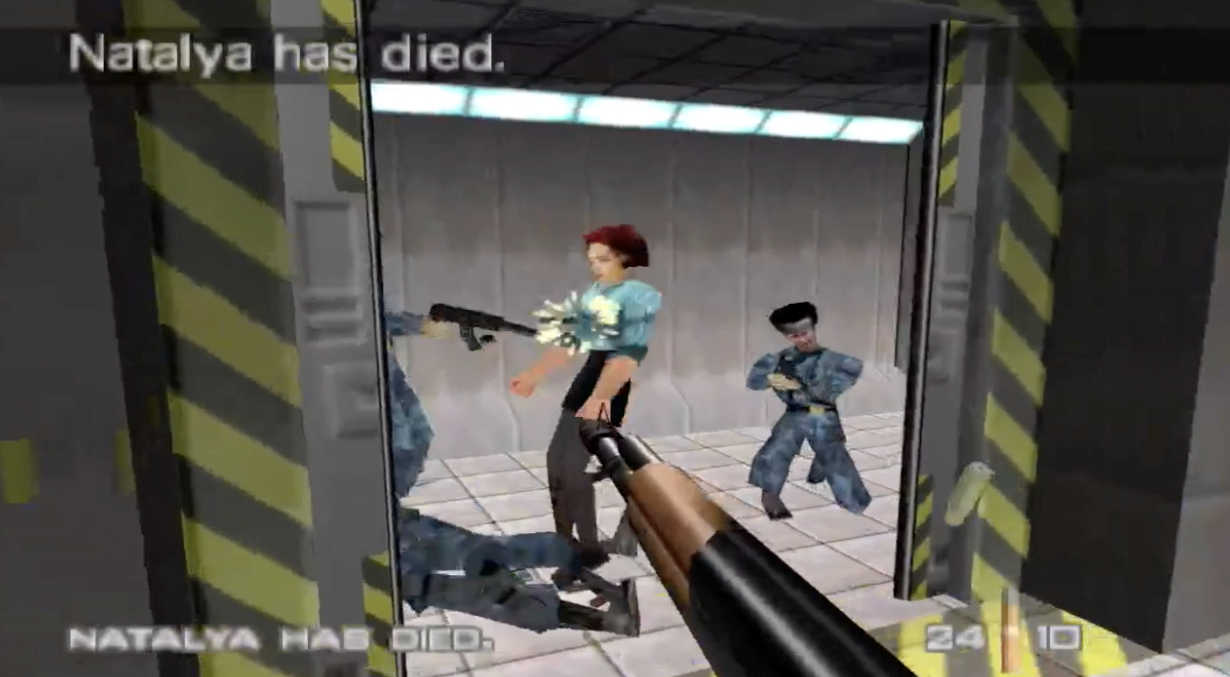
\includegraphics[width=0.60\columnwidth]{images/natalya.png}%
		\caption{Natalya, regrettant sa décision de se jeter au milieu de PNJ hostiles}%
	\end{center}
\end{figure}

\newpage
\subsection{Entre la sérendipité et l'apophénie}

De par son côté évolutif et de plus en plus complexe, il est parfois difficile de prévoir tous les résultats possibles d’une interaction enter le joueur et l’IA, ce qui donne parfois lieu à ce que l'on pourrait appeler des expériences émergentes, avec des PNJ au comportement imprévisible, même pour les créateurs.

Si dans les jeux, cet aspect peut presque passer inaperçu et n'est pas très présent, comme dans Fable, il s'agit d'une des principales fonctionnalités de certains programmes, comme le chatbot Evie (Evie n'est pas un jeu vidéo au sens classique du terme, mais cela reste un programme ludique avec lequel le joueur peut interagir).

\newpage
\subsubsection{Fable, un monde plus vivant qu'il n'y paraît}

Fable est un jeu sorti en 2004, et innovant pour son époque, de par la liberté qu’il laisse au joueur. En effet, le joueur peut se marier, divorcer, boire, jouer aux cartes, acheter, louer et revendre des maisons, se tourner vers les forces obscures ou le bien, massacrer des innocents, gardes ou bandits, entre autres activités diverses et variées.

Ce qui suit est une anecdote tirée du blog d’un des développeurs du jeu\cite{fable}, traduite, adaptée et commentée.

%Les développeurs se sont également imposés deux règles qu’ils jugeaient vitales que le jeu suive, sans quoi il ne respecterait pas leur vision :
%
%\begin{itemize}
%	\item Le monde dans lequel le joueur évolue, ainsi que tous ses occupants doivent réagir de manière appropriée aux actions du joueur.
%	\item Le personnage principal doit exprimer visuellement ce qu’il ressent.
%\end{itemize}
	
\textbf{Un monde simulé}

Pour rendre le monde plus intéressant, les développeurs ont donné à chaque PNJ leurs propres traits de caractères.

%\begin{wrapfigure}{r}{0.4\textwidth}
%	\begin{center}
%		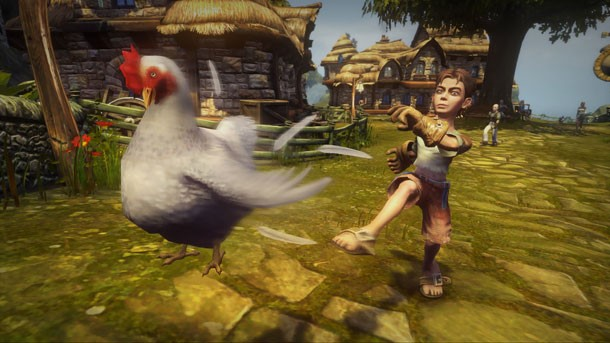
\includegraphics[width=0.38\textwidth]{images/chicken.jpg}
%	\end{center}
%	\caption{Enfant tourmentant une poule dans Fable}
%\end{wrapfigure}

Ils ont également remarqué que les joueurs étaient particulièrement sensibles aux émotions des enfants. Ils ont donc décidé de rendre le comportement des enfants très varié. Ainsi, certains sont de véritables petites pestes, et s'amusent en tourmentant des poules, tandis que d’autres vont à l’école bien en rangs, et rentrent gentiment à la maison à l’heure pour le goûter.

Et, peut-être le plus important, les enfants fixeront avec intensité ce qu’ils trouvent intriguant.

\begin{figure}[!h]%
	\begin{center} 
		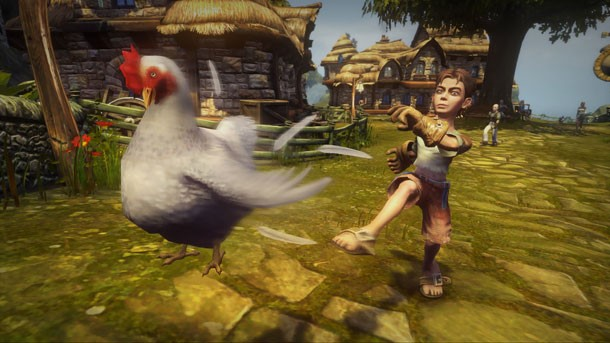
\includegraphics[width=0.40\columnwidth]{images/chicken.jpg}%
		\caption{Enfant tourmentant une poule dans Fable}%
	\end{center}
\end{figure}

\textbf{Un héros expressif}

Plutôt que d’afficher plein de caractéristiques comme dans un RPG classique, les développeurs ont trouvé plus intéressant de montrer par des mouvements et des expressions que le personnage réagit au monde qui l’entoure (plutôt que de rester planter là, sans émotions apparentes).

\newpage
\textbf{Un héros expressif dans un monde simulé}

%Quand on mélange les deux, voici ce que cela peut donner :

Imaginez-vous la scène, une radieuse journée à Bowerstone (une ville du jeu). Les papillons papillonnent, le parfum des tulipes vous est porté par une brise. Au loin, on entend des enfants jouant et rigolant dans une cour de récréation, réticent à retourner en classe, malgré le son de cloche qui signifie la fin de la pause.

Le cours a repris, après quelques remontrances de l’institutrice. Un des enfants, trouvant le cours assommant, regarde par la fenêtre en soupirant.

Un homme s’infiltre silencieusement dans l’école. L’institutrice lui tourne le dos. Elle ne se doute de rien.

Un par un, les enfants se mettent à fixer quelque chose derrière l’institutrice. La classe devient silencieuse. Finalement, l’institutrice entend un bruit derrière elle, se retourne et …

… tombe nez à nez avec un homme en caleçon, planté au milieu de sa salle de classe, souriant à pleines dents. Soudain, souriant de plus belle, il fait un doigt d’honneur. Tout le monde hurle …

\textbf{Ce qu'il s'est vraiment passé}
\begin{itemize}
	\item Le personnage sourit car il se sent sécurité.
	\item Les enfants fixent ce qui leur semble intéressant (ici, le personnage, qui est une nouveauté pour eux).
	\item Le doigt d’honneur est considéré comme un acte d’agression, d’où les cris.
\end{itemize}	

On pourrait ici presque parler de « comportement émergent » (en parallèle au gameplay émergent, dans lequel les joueurs trouvent de nouvelles façons de jouer que les développeurs n’avaient pas prévu) car en partant de règles simples, on arrive à une situation complexe et crédible.

C’est également un bon exemple d’apophénie (fait de donner un sens particulier à des évènements banals), puisque le joueur interprète les réactions des PNJ différemment de ce que les développeurs avaient probablement en tête lors de la réalisation du jeu. 

\newpage
\subsubsection{De ELIZA à Evie}

Un agent conversationnel (ou chatbot en anglais), est un logiciel autonome qui a pour fonction de dialoguer avec l’utilisateur. Pour cela, la phrase entrée par l’utilisateur est traduite en un langage intermédiaire pour permettre à l’agent de l’analyser, qui va ensuite générer une réponse plus ou moins appropriée.

ELIZA, créé en 1966, par Joseph Weizenbaum, MIT, fut le premier agent conversationnel développé. Son comportement était très simple et fixé à l'avance (elle répondait aux questions en demandant pourquoi cette question, si elle détectait le mot « ordinateur », elle demandait si la question lui avait été posée parce qu’elle même est une machine), et laissait donc peu de place à une vraie conversation.

\begin{figure}[!h]%
	\begin{center} 
		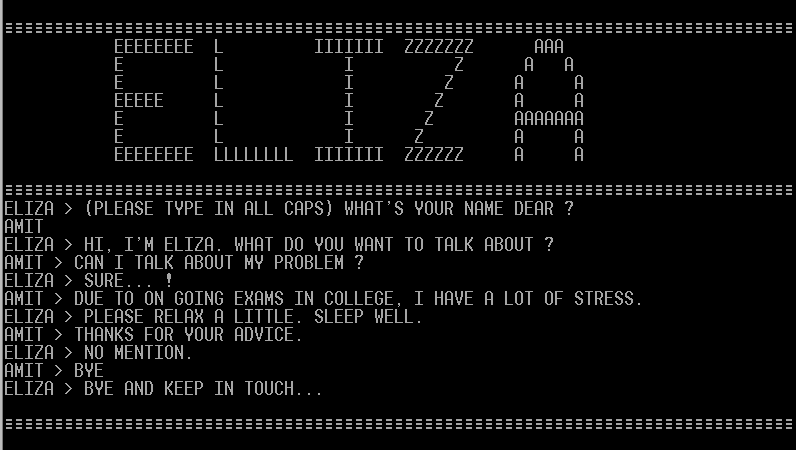
\includegraphics[width=0.50\columnwidth]{images/eliza.png}%
		\caption{ELIZA, premier chatbot}%
	\end{center}
\end{figure}

En 1997, Rollo Carpenter, un informaticien britannique, crée Jabberwacky. C’est lui aussi un agent conversationnel, mais au lieu d’avoir un comportement fixé à l'avance, celui-ci est capable d’apprendre. En effet, il stocke dans une base de données toutes les conversations des utilisateurs, et s’en sert pour choisir une réponse à la question posée par l’utilisateur.

Ce n’est que onze ans plus tard, en 2008 que Rollo Carpenter met en ligne Cleverbot\cite{carpenter2011cleverbot}, descendant spirituel de Jabberwacky. Celui-ci dispose également d’une base de données des conversations avec les utilisateurs parmi lesquelles il va chercher la réponse la plus appropriée, mais a également une notion de contexte, grâce à un système de mémoire à court terme, qui donne un poids plus important aux conversations récentes.

%\newpage
%\begin{figure}[!h]%
%	\begin{center} 
%		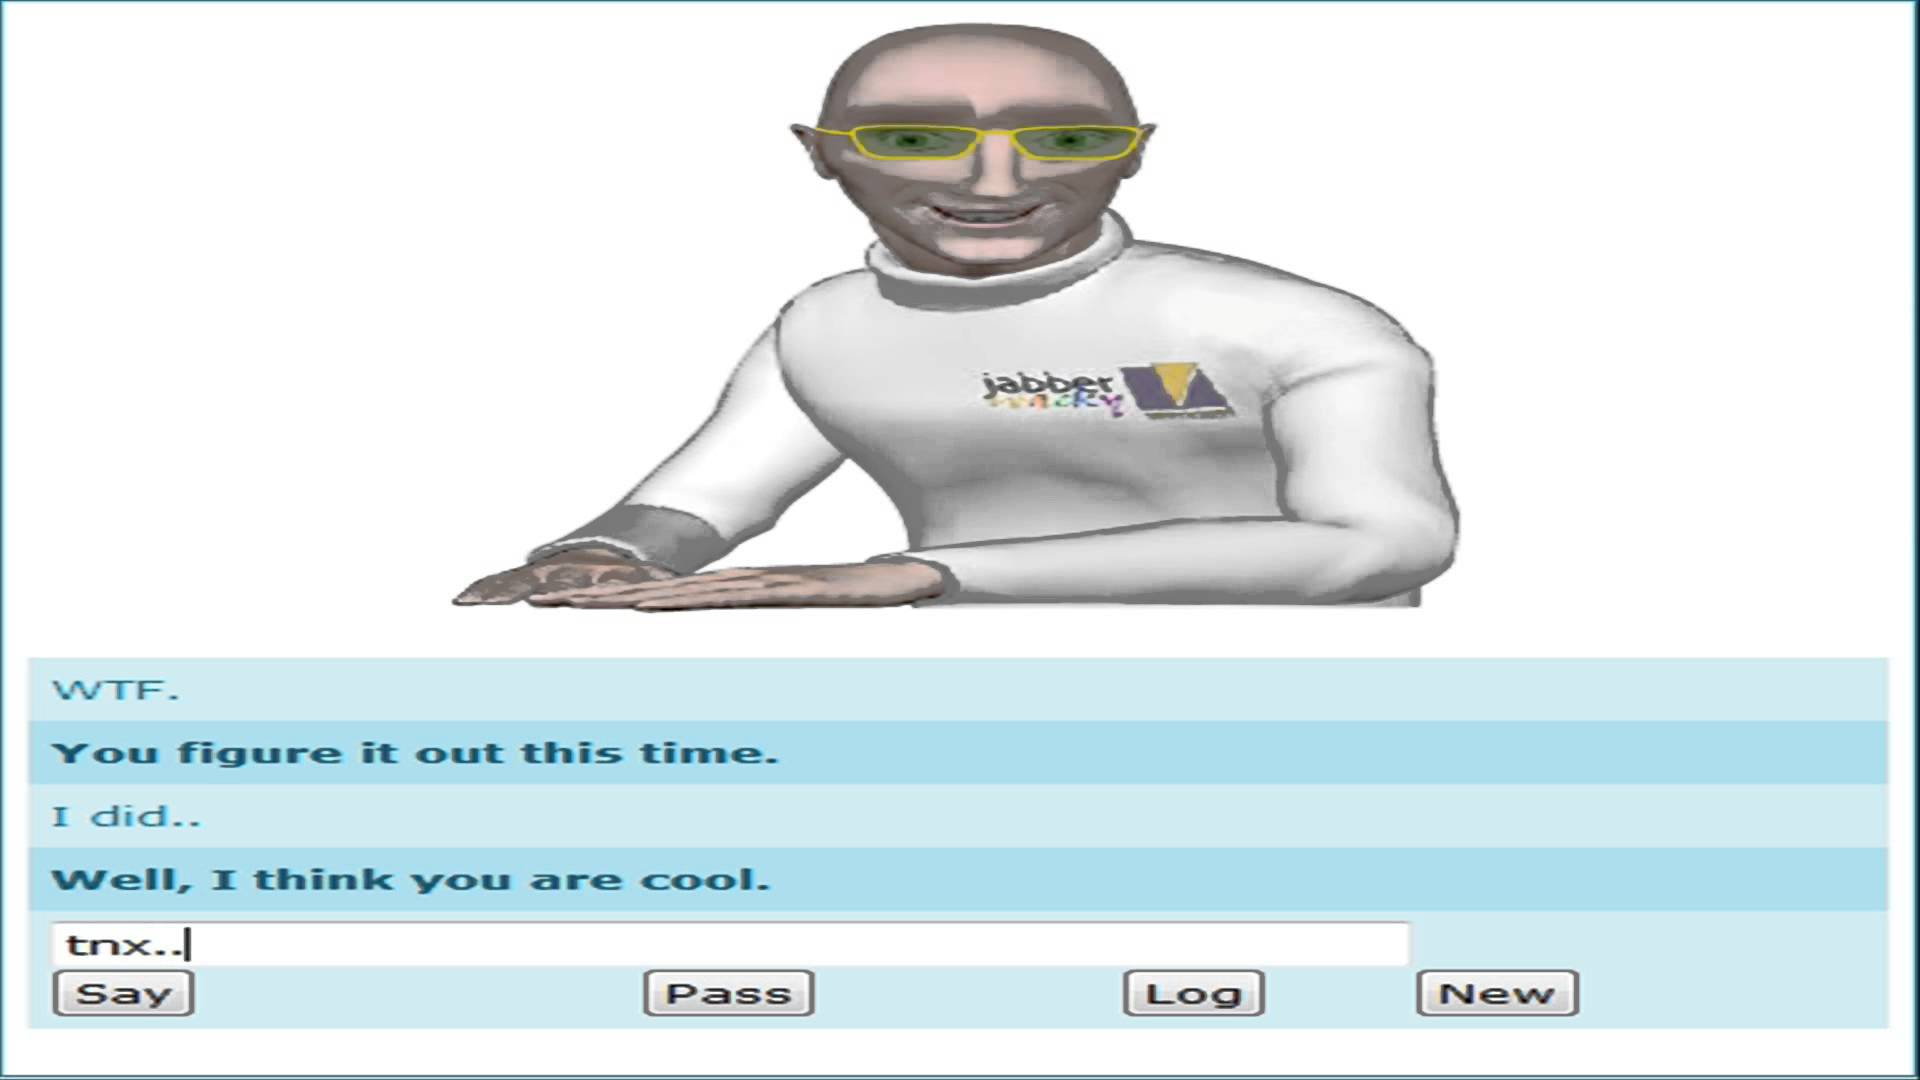
\includegraphics[width=0.60\columnwidth]{images/jabberwacky.jpg}%
%		\caption{Jabberwacky, en pleine discussion}%
%	\end{center}
%\end{figure}

C'est également à ce moment que Existor voit le jour, fondée par Rollo Carpenter, entreprise qui se donne pour objectif de créer des algorithmes pour arriver à un niveau de conversation humaine naturelle.

Ainsi, c’est en 2015 que Evie (\textbf{E}lectronic \textbf{V}irtual \textbf{I}nteractive \textbf{E}ntity), la petite sœur de Cleverbot, voit le jour. Devant la quantité de données que les différents chatbot de Existor récoltent chaque jour (5,5 millions de conversations par jour), et le nombre impressionnant de 1,5 milliards de conversations enregistrées, les développeurs de Existor décident d'utiliser des techniques de Machine Learning pour les analyser. 

\begin{figure}[!h]%
	\begin{center} 
		
\includegraphics[width=0.40\columnwidth]{images/evie.png}%
		\caption{Evie}%
	\end{center}
\end{figure}

Dans un premier temps, ils cherchent  des motifs récurrents dans les phrases, puis, à l’aide de RNNLM (\textbf{R}ecurrent \textbf{N}eural \textbf{N}etwork \textbf{L}anguage \textbf{M}odels), ils arrivent à  estimer les probabilités qu'un mot en suive un autre, afin de former une phrase plus naturelle.

Cette expérience se rapproche alors de la sérendipité, qui à l'origine désigne le fait de réaliser une découverte scientifique inattendue dans le cadre d'une recherche concernant un autre sujet. Toutefois, le sens du terme est aujourd'hui plus large, englobant ainsi la navigation sur internet, qui peut en quelques liens nous emmener dans des endroits complètement inattendus.

Ainsi, même si les réponses de Evie sont de plus en plus naturelles, le joueur ne sait jamais trop jusqu'où une conversation avec elle peut aller. Comme dans une discussion naturelle, le sujet change au fur et à mesure de la conversation, parfois de manière brusque quand Evie ne comprend pas bien la phrase du joueur, et le joueur peut très vite se retrouver dans une situation dans laquelle Evie l'insulte sans raison, ou en train de se battre pour avoir le dernier mot.

%------------------------------------------------

\newpage
\section{Apports du mémoire}

Lors de nos recherches pour écrire ce mémoire, nous avons non seulement approfondi énormément nos connaissances sur beaucoup de sujets qui touchent à l'intelligence artificielle, notamment le machine learning, cependant, il s'agit d'un sujet tellement vaste que nous n'avons pas pu aborder toutes les approches qui existent.

Nous avons également découvert plusieurs applications dont nous n'avions aucune idée de l'existence, comme Angelina, l'IA qui développe des jeux.

Lors du développement de nos prochains jeux, nous aurons ainsi une meilleure idée de ce qu'il est possible d'utiliser puisque nous nous serons déjà familiarisé avec une grande partie des techniques qui sont utilisées dans le monde du jeu vidéo, mais également avec des techniques naissantes.

%------------------------------------------------

\newpage
\section{Conclusion}

Ainsi nous avons vu qu'à ses débuts, l'intelligence artificielle dans les jeux vidéo était très limitée, et qu'on ne pouvait même pas vraiment parler d'intelligence, mais plutôt de « réaction programmée à une action donnée ». Mais très vite, des jeux comme F.E.A.R. ou Black \& White vont apparaître et montrer de nouvelles techniques et applications pour le jeu vidéo.

Nous avons vu que les applications pour l'IA dans le monde du jeu vidéo étaient nombreuses, avec notamment le Machine Learning, domaine extrêmement vaste et prometteur pour les jeux vidéo, encore jeune mais de plus en plus utilisé, en nous attardant seulement sur les réseaux de neurones (utilisées dans rtNEAT), et les arbres de comportement, très couramment utilisées pour des PNJ avec un comportement fixé à l'avance.

Mais aussi, le Dynamic Game Difficulty Balancing, qui permet d'offrir une expérience plus adaptée, et parfois plus personnalisée, au joueur, en modifiant à la volée certains éléments du jeu.
Sans oublier les IA capables d'apprendre à jouer, tandis que d'autres, à partir d'une description de quelques dizaines de lignes, peuvent créer un jeu.

Enfin, nous avons aussi vu une autre utilité à l'intelligence artificielle, celle de garder le joueur immergé dans l'univers du jeu. Pour cela, il est vital de ne pas rompre la suspension consentie de l'incrédulité de joueur et d'éviter de lui faire ressentir tout sentiment de solipsisme. 
Nous avons également remarqué que l'apophénie peut être un bon moyen d'améliorer l'immersion du joueur, tandis que la sérendipité permet d'augmenter considérablement la durée de vie du jeu, le joueur ne sachant jamais ce qui l'attend.

%----------------------------------------------------------------------------------------
%	BIBLIOGRAPHY
%----------------------------------------------------------------------------------------
\newpage
\bibliographystyle{unsrt}
\bibliography{References}

%----------------------------------------------------------------------------------------

\end{document}
